%%%% ijcai19-multiauthor.tex

\typeout{IJCAI-19 Multiple authors example}

% These are the instructions for authors for IJCAI-19.

\documentclass{article}
\pdfpagewidth=8.5in
\pdfpageheight=11in
% The file ijcai19.sty is NOT the same than previous years'
\usepackage{ijcai19}

% Use the postscript times font!
\usepackage{times}
\usepackage{soul}
\usepackage{url}
\usepackage[hidelinks]{hyperref}
\usepackage[utf8]{inputenc}
\usepackage[small]{caption}
\usepackage{graphicx}
\usepackage{amsmath}
\usepackage{booktabs}
\urlstyle{same}

\usepackage{wrapfig}

%%%%%%%%%%%%% ADD CUSTOM PACKAGES TO macros.sty
\usepackage{macros}



\newcommand{\colalg}{{\tt ColAlg}}
\newcommand{\expthree}{{\tt Exp3}}
\newcommand{\latentranker}{{\tt LRB}}
\newcommand{\rowalg}{{\tt RowAlg}}
\newcommand{\ucb}{{\tt UCB1}}
\newcommand{\ucbe}{{\tt UCB1\mbox{-}Elim}}
\newcommand{\linucb}{{\tt LinUCB}}
\newcommand{\glmucb}{\tt GLM-UCB}
\newcommand{\rankelim}{\tt Rank1-Elim}


\newcommand{\RBAEXP}{{\tt RBA-EXP3}}
\newcommand{\RBA}{{\tt RBA}}
\newcommand{\RBAUCB}{{\tt RBA-UCB1}}
\newcommand{\LRAUCB}{{\tt LRA-UCB1}}
\newcommand{\LRAEXP}{{\tt LRA-EXP3}}
\newcommand{\LRATS}{{\tt LRA-TS}}
\newcommand{\NMFBan}{{\tt NMF-Ban}}
\newcommand{\WMA}{{\tt WMA}}


%%%%%%%%%%%%%For adding comments

\newcommand{\todob}[2][]{\todo[color=cyan!20,size=\tiny,inline,#1]{B: #2}} % Brano's comments
\newcommand{\todosb}[2][]{\todo[color=green!20,size=\tiny,inline, #1]{S: #2}} %
\newcommand{\todoan}[2][]{\todo[color=black!20,size=\tiny,inline, #1]{A: #2}} %

% the following package is optional:
%\usepackage{latexsym} 

% Following comment is from ijcai97-submit.tex:
% The preparation of these files was supported by Schlumberger Palo Alto
% Research, AT\&T Bell Laboratories, and Morgan Kaufmann Publishers.
% Shirley Jowell, of Morgan Kaufmann Publishers, and Peter F.
% Patel-Schneider, of AT\&T Bell Laboratories collaborated on their
% preparation.

% These instructions can be modified and used in other conferences as long
% as credit to the authors and supporting agencies is retained, this notice
% is not changed, and further modification or reuse is not restricted.
% Neither Shirley Jowell nor Peter F. Patel-Schneider can be listed as
% contacts for providing assistance without their prior permission.

% To use for other conferences, change references to files and the
% conference appropriate and use other authors, contacts, publishers, and
% organizations.
% Also change the deadline and address for returning papers and the length and
% page charge instructions.
% Put where the files are available in the appropriate places.

\title{Non-stochastic Low Rank Bandit}

\author{Author names withheld}

\begin{document}

\maketitle
\begin{abstract}
We study the problem of learning the maximum entry of a low-rank non-negative matrix, from sequential observations. In this setting, the learner chooses tuples of rows and columns at every round and observes the corresponding submatrix. The main challenge in this setting is that the learner does not observe the individual latent values of rows and columns as its feedback. Diverging from previous works, we assume that the preference matrix is non-stochastic and hence our setting is more general in nature. Existing methods for solving similar problems rely on UCB-type algorithms based on constructing conservative confidence intervals with the strong assumption that underlying distributions are stochastic. We depart from this standard approach and consider the case when the best row and column pair can be learned jointly with the help of two separate bandit algorithms working individually on rows and columns. We propose a simple and computationally efficient algorithm that implements this procedure, which we call Low Rank Bandit, and prove a sub-linear bound on its $n$-step regret in the rank-$1$ special case. We evaluate the algorithm empirically on several synthetic and real-world datasets. In all experiments, we outperform existing state-of-the-art algorithms. \todoan{Should we say 'existing state-of-the-art algorithms adapted to this setting'?}
\end{abstract}

\section{Introduction}
\label{sec:introduction}
%!TEX root = paper.tex

In this work, we study the problem of learning personalized ranked lists of diverse items for multiple users, from sequential observations of user preferences. We are interested in utilizing latent similarities among users and items to learn these lists much faster than learning a separate ranked list for each user. The key structure in our problem is that the user-item preference matrix is low rank, which is a standard assumption in recommender systems \citep{koren2009matrix,ricci2011liorrokach}. The learning agent has access to noisy observations of the user-item matrix. It does not have access to either user or item latent factors.

We formalize our learning problem as the following online learning problem. At time $t$, a random user $i_t$ from a pool of $K$ users arrives to the recommender system. The learning agent observes the identity of the user $i_t$, recommends a list of $d$ diverse items $J_t$ from a pool of $L$ items as a response, and observes the preferences of user $i_t$ for all recommended items $J_t$. The user-item preference matrix is low-rank at each time $t$, can vary substantially over time, and does not have to be stochastic. The reward of the recommended list is high when highly preferred items of the user are recommended at higher positions. The goal of our learning agent is to compete with the most rewarding diverse list for each user in hindsight.

Our learning model is motivated by a real-world scenario, where the learning agent suggests movies to users and each movie belongs to different movie genres. The agent typically does not observe instantaneous preferences of the user, and therefore suggests multiple movies that may be of interest to the user under different circumstances. A similar model has also been studied in \citet{carbonell1998use} where the goal is to suggest a diversified list to each incoming user that combines relevance to the query as well as novelty. The authors suggest an approach where each item in the list is relevant to the query but also has \textit{"marginal relevance"} or less similarity with previously selected documents and this improves the quality of recommendation.


\todob{This is actually the main motivation for diversity. We need to add proper references and discuss this in detail.}

\todosb{I wrote about main motivation behind diversity }

We make four major contributions. First, we formulate our online learning problem as a latent ranked bandit on low-rank matrices. We identify a family of non-negative low-rank matrices where our problem can be solved statistically efficiently, without estimating the latent factors of the user-item preference matrix. The key structure of our matrix is that the set of optimal items of all users is small and can be learned jointly for all users. Given these items, the problem of learning the optimal order for each user can be solved in the full-information setting and thus is easy. Second, we propose a computationally-efficient algorithm that implements this idea, which we call latent ranker algorithm ($\latentranker$). The algorithm has two components, column learning and row ranking, which learn the set of optimal items of all users and then sort them, respectively. The column learning algorithm is similar to ranked bandits. In particular, we learn the $k$-th most diverse item using a multi-armed bandit, whose rewards are conditioned on the rewards of $k - 1$ previously chosen items. The row learning problem is solved separately for each user. Because it is in the full-information setting, as we observe the individual rewards of all recommended items,  we solve it using the weighted majority algorithm. Third, we analyze $\latentranker$ and up to problem-specific factors, we prove a $O\left(d \sqrt{L n} + K \log n + K d \log d\right)$ upper bound on its $n$-step regret. The regret of a naive solution is $O(\sqrt{K L n})$, and is much worse than that of $\latentranker$ when all of $K$, $L$, and $n$ are large. Finally, we evaluate $\latentranker$ empirically on several synthetic and real-world problems. Perhaps surprisingly, $\latentranker$ performs well even when our modeling assumptions are violated.

The paper is organized as follows. We introduce necessary background to understand our work in \cref{sec:background} and define our online learning problem in \cref{sec:setting}. We propose our algorithm in \cref{sec:algorithm} and bound its regret in \cref{sec:analysis}. In \cref{sec:experiments}, we evaluate the algorithm empirically. In \cref{sec:related work}, we survey related work. We conclude in \cref{sec:conclusions}. The detailed proof of our regret bound is presented in \cref{sec:proof}.


\section{Rank-$1$ Background and Setting}
\label{sec:background}
%!TEX root = bandit_paper.tex

\newcommand{\transpose}{^\mathsf{\scriptscriptstyle T}}
\textbf{Notations:} We denote $[n] = \{1, \dots, n\}$ as the set of the first $n$ positive integers. Let $M$ denote any arbitrary matrix of size $m \times n$ matrix. Let the rank of the matrix be denoted by $d$. We denote by $A^B$ the set of all vectors whose entries take values from set $A$ and are indexed by set $B$, where $A$ and $B$ can be any arbitrary sets. For any $d$ and $I \in [m]^d$, $M(I, :)$ denotes a $d \times n$ submatrix of $M$ whose $i$-th row is $M(I(i), :)$. Similarly, for any $d$ and $J \in [n]^d$, $M(:, J)$ denotes a $m \times d$ submatrix of $M$ whose $j$-th column is $M(:, J(j))$. Finally, we denote $\Pi_d$ as the set of all $d$-permutations. For an element $\pi \in \Pi_d$ and $d$-dimensional vector $v$, we denote by $\pi(v)$ the permutation of the entries of $v$ according to $\pi$.
%We index the rows and columns of the matrices by vectors.
%\todob{The previous sentence does not make any sense. What is the set of size $m \times n$?}
%\todoan{We don't index the rows and columns by vectors, but define what it means to use vector indexing. You can just remove this sentence.}

\textbf{Rank-$1$ Setting:} We study the online learning problem of finding the maximum entry of a family of non-stochastic, low-rank and non-negative matrices  which we call as the \emph{non-stochastic low-rank bandit problem}. We first analyze the simple rank-$1$ setup and propose our solution for this setting. Many of the key aspects of our design principle are captured in this rank-$1$ setting. Let $U_t\in [0,1]^{K\times 1}$ be the row preference over a single topic and $V_t \in [0,1]^{L\times 1}$ be the column preference over a single topic. The row-column \emph{preference matrix} $M_t = U_tV_t^{\intercal}$ is non-negative, non-stochastic, and rank $1$. We assume that,
\begin{align}
i^\ast = \argmax_{i\in[K], t\in[n]}U_t(i,1), \hspace{1.5em}
j^\ast = \argmax_{j\in[L], t\in[n]}V_t(j,1) \label{eq:rank1ij}.
\end{align}
Thus, this assumption makes sure that the row and column preferences ($U_t$ and $V_t$ respectively) can change with time $t$, but the best row and column does not change over all time $t\in[n]$. At every round $t$, the learner chooses one pair of row and column indexed by $i_t$ and $j_t$ respectively and observes their product $U_t(i_t)V_t(i_t)$ as its feedback.
%\todob{You make it sound like there is only one matrix. This is false.}
%Note, that we refer to the rows as rows and to the columns as columns because this is a standard terminology in recommender systems, where we envision applications of our work.

\textbf{Regret Definition (Rank-$1$):} The goal of the learner is to minimize the expected $n$-step regret with respect to the optimal solution in the hindsight as follows,
\begin{align}
  R(n) =
  \sum_{t = 1}^n \E\left[M_t(i^\ast, j^\ast) - M_t(i_t,j_t)\right]\,
  \label{eq:regret}
\end{align}
where, the expectation is over any random choice of rows and columns. 

%\todob{Please do not use non-standard notation. $\{\}$ is a set!!! You want to write either $\argmax_{i \in [K], \, t \in [n]} U_t(i, 1)$ or $\argmax_{(i, t) \in [K] \times [n]} U_t(i, 1)$. You also need to move this earlier. You want to say that the best row and column does not change over time.}

%At time $t$, the preferences of users over columns are encoded in a $K \times L$ \emph{preference matrix} $M_t = U_t V_t\transpose$, where $M$, where  the rank of $M$ is $d=1$.
%$U_t$, and $V_t$ are defined as in \cref{sec:background}
%Note that for $d=1$, 

%We study the online learning problem of finding the maximum entry of a non-stochastic, low-rank and non-negative matrix $M$ which we call as a \emph{non-stochastic low-rank bandit problem}. At time $t$, the preferences of users over columns are encoded in a $K \times L$ \emph{preference matrix} $M_t = U_t V_t\transpose$, where $M$, $U_t$, and $V_t$ are defined as in \cref{sec:background}. We assume that row and column preferences ($U_t$ and $V_t$ respectively) can change with time $t$. At every timestep $t$ the learner chooses one pair of row and column indexed by $i_t$ and $j_t$ and observes their product $U_t(i_t)V_t(i_t)$ as its feedback.



%Let $\Pi_d$ be the set of all $d$-permutations. For any $\pi \in \Pi_d$ and $d$-dimensional vector $v$, we denote by $\pi(v)$ the permutation of the entries of $v$ according to $\pi$.

%\todob{This section seems like an exact copy of the arxiv paper. Please change language. Otherwise we may be accused of plagiarism.}

%\textbf{Hott-topics Assumption:} We focus on a family of low-rank matrices, which are known as hott topics. We define a \emph{hott-topics matrix} of rank $d$ as $M = U V\transpose$, where $U$ is a $K \times d$ non-negative matrix and $V$ is a $L \times d$ non-negative matrix that gives rise to the hott-topics structure. In particular, we assume that there exists $d$ rows $I^\ast$ in $U$ such that each row in $U$ can be represented as a convex combination of rows of $I^\ast$ and the zero vector. Hence, for an $A = \{a \in [0, 1]^{d \times 1}: \|a\|_1 \leq 1\}$ each row of $U$ can be expressed as,
%\begin{align}
%  \forall i \in [K] \ \exists \alpha \in A: U(I^\ast, :) \alpha = U(i, :)\,,
%  \label{eq:hott topics1}
%\end{align}
%Similarly, we assume that there exist $d$ rows $J^\ast$ in $V$ such that each row of $V$ can be expressed as a convex combination of rows $J^\ast$ and the zero vector,
%\begin{align}
%  \forall j \in [L] \ \exists \alpha \in A: V(J^\ast, :) \alpha = V(j, :)\,,
%  \label{eq:hott topics}
%\end{align}
%where $A = \{a \in [0, 1]^{d \times 1}: \|a\|_1 \leq 1\}$. Note that we refer to the rows as users and to the columns as columns because this is a standard terminology in recommender systems, where we envision applications of our work. Hence, the matrix $M$ represents preferences of users for columns, $M(i, j)$ is the preference of user $i$ for column $j$. The rank $d$ of $M$ is the number of latent topics. The matrix $U$ are latent preferences of $K$ users over $d$ topics, where $U(i, :)$ are the preferences of user $i \in [K]$. The matrix $V$ are latent preferences of $L$ columns in the space of $d$ topics, where $V(j, :)$ are the coordinates of column $j \in [L]$. Without loss of generality, we assume that $U \in [0, 1]^{K \times d}$ and $V \in [0, 1]^{L \times d}$. We assume that the coordinates are points in a simplex, that is $\|U(i, :)\|_1 \leq 1$ for all $i \in [K]$ and $\|V(j, :)\|_1 \leq 1$ for all $j \in [L]$. Note that our assumptions imply that $M(i, j) \geq 0$ for any $i \in [K]$ and $j \in [L]$.

%\todob{We say that the rows are users and that the columns are columns. But they do not have to be, right? Say that we refer to the rows as users and to the columns as columns because this is a standard terminology in recommender systems, where we envision applications of our work.}


\section{Rank-$1$ Algorithm}
\label{sec:rank1}
%!TEX root = bandit_paper.tex

%We first analyze the simple rank $1$ scenario and propose our solution for this setting. Many of the key aspects of our design principle are captured in this rank-$1$ setting. Note that for $d=1$, $U_t\in [0,1]^{K\times 1}$ is the user preference over a single topic and $V_t \in [0,1]^{L\times 1}$ is the item preference over a single topic. The user-item preference matrix $M_t = U_tV_t^{\intercal}$ is non-negative, non-stochastic, and rank $1$. 


%Also, the hott-topics assumption in eq \eqref{eq:hott topics1} and \eqref{eq:hott topics} still holds in the rank $1$ setting.  In this setting, at every timestep $t\in[n]$ the learner selects a pair of rows and columns, denoted by $i_t$ and $j_t$ respectively and observes the feedback $M_t(i_t,j_t)$.
%
%\todob{Explain why.}
%\todob{Use \textbackslash eqref when referring to equations.}

We present the simple \todob{Avoid repetitive use of ``simple''. You make it sound like we do only easy things.} algorithm Low Rank Bandit $\latentranker$ \todob{Confusing. A name followed by its abbreviation.} in Algorithm \ref{alg:LRB} for the rank $1$ setting. The $\latentranker$ consist of two key components, a row learning algorithm and a column learning algorithm. At every round $t$ the row algorithm suggest the row $i_t \in [K]$ and the column algorithm suggests the column $j_t\in [L]$. Note, that in this non-stochastic scenario we use $\expthree$ as the row and column learning algorithm. The row $\expthree$ has $K$ arms and the column $\expthree$ has $L$ arms. The main idea is to use the row $\expthree$ to learn the best row on average while the column $\expthree$ learns the best column on average. The learner then observes the reward $M_t(i_t, j_t)$ and updates the row and column $\expthree$ simultaneously. A key insight to this simple design is that when both the row and column learner are run simultaneously, they will learn the most rewarding row and column on average and converge on the maximum entry of the the matrix $M$. From the definition of $U_t$, for any sequence of $n$ columns, the maximum value is in row $i^\ast$. \todob{This property of $U_t$ and $V_t$ needs to stated formally. They cannot be arbitrary, as you claimed earlier.} This means that the row algorithm learns irrespective of what the column algorithm does. From the definition of $V_t$, for any sequence of $n$ rows, the maximum value is in column $j^\ast$. \todob{Again, this property of $U_t$ and $V_t$ needs to stated formally. They cannot be arbitrary, as you claimed earlier.} This means that the column algorithm learns irrespective of what the row algorithm does.

%\todob{Use ``round'' instead of time, timestep, step, and such.}

%\todob{We need to clearly explain what is going on here. From the definition of $U_t$, for any sequence of $n$ columns, the maximum value is in row $i^\ast$. This means that the row algorithm learns no matter what the column algorithm does. From the definition of $V_t$, for any sequence of $n$ rows, the maximum value is in column $j^\ast$. This means that the column algorithm learns no matter what the row algorithm does.}

\begin{algorithm}[t]
  \caption{Low Rank Bandit ($\latentranker$) (Rank-$1$)}
  \label{alg:LRB}
  \begin{algorithmic}[1]
    \State \textbf{Input:} Time horizon $n$
    \Comment{Initialization}
      \State Initialize $\rowalg $
      \State Initialize $\colalg $
    \For{$t = 1, \dots, n$}
      \Comment{Generate response}
        \State Row $i_t$ suggested by $\rowalg$
        \State Column $j_t$ suggested by $\colalg$
        \State Observe $M_t(i_t, j_t)$
      \Comment{Update statistics}
    \State Update arm $i_t$ of $\rowalg$ with reward $M_t(i_t, j_t)$.
    \State Update arm $j_t$ of $\colalg$ with reward $M_t(i_t, j_t)$.
     \EndFor
  \end{algorithmic}
\end{algorithm}


\vspace*{-0.5em}
\section{Analysis of Rank-$1$ Setting}
\label{sec:analysis}
%!TEX root = bandit_paper.tex

\begin{theorem} \textbf{(Rank-1 Case)}
\label{thm:upper bound} Let $\colalg$ and $\rowalg$ in $\latentranker$ be $\expthree$ algorithm, respectively. Then the expected $n$-step regret of $\latentranker$ is bounded as
\begin{align*}
  R(n) = O\left(\frac{\left(\sqrt{L } + \sqrt{K }\right)\sqrt{n}}{\alpha}\right)
\end{align*}
where $\alpha > 0$ is such a lower bound that for all $i\in[K], j\in [L]$ and $t \in [n]$, $U_{t}(i,1) > \alpha$ and $V_{t}(j,1) > \alpha$.
%where $\alpha = \min_{t \in [n]} \min_{i_t,j_t:\ , i_t \neq i^*_t \, j_t \neq j^*_t} \E\left[u_t(i^*_t)v_t(j^*_t)\right] - \E\left[u_t(i_t)v_t(j_t)\right]$ \todob{I do not think that this definition of $\Delta$ is correct. If you look into the proof, you will note that $\Delta$ there has nothing to do with the gap. We should not call this quantity $\Delta$ because this will confuse reviewers.} is an instance-specific lower bound on the gap in the expected rewards of the optimal and best suboptimal columns and rows at any time $t \in [n]$, averaged over all users at that time.  

%\todob{We need to define the unweighted reward.}

\end{theorem}
\begin{proof}
Let, $(u_t v_t\transpose)_{t = 1}^n$ be a sequence of $n$ non-negative rank-$1$  matrices such that $u_t \in [0, 1]^{K \times 1}, v_t \in [0, 1]^{L \times 1}$, and the highest entry is $(1, 1)$. Let,
\begin{align*}
((i_t, j_t))_{t = 1}^n
\end{align*}
be a sequence of $n$ row-column pairs chosen by a learning agent. Then the expected n-step regret of the agent is,

%\todob{Properly write numbers and symbols. This should be ``$n$ non-negative rank-$1$''.}
%\todob{Properly bracket expectations. Lack of brackets repeats throughout the proof.}

\begin{align*}
R(n) = \sum_{t = 1}^n \E \left[{u_t(1) v_t(1) - u_t(i_t) v_t(j_t)}\right]
\end{align*}
where the expectation is over the randomness of the agent. Now note that for any $u$, $v$, $i$, and $j$ in our problem we can show that,
\begin{align*}
& 2 (u(1) v(1) - u(i) v(j))\\
& = \!\! 2 u(1) v(1) \! - \! u(i) v(1) \! - \! u(1) v(j) \! + \! u(i) v(1) \! + \! u(1) v(j) \! - \! 2 u(i) v(j) \\
& = u(1) (v(1) - v(j))  + v(1) (u(1) -  u(i))  +\\
& \hspace*{3em}  u(i) (v(1)  - v(j))  + v(j) (u(1)  - u(i)) \\
%& = \!\! u(1) (v(1)\! - \! v(j)) \! + \! v(1) (u(1) \!- \! u(i)) \! +\\
%& \! u(i) (v(1) \! -\! v(j)) \! +\! v(j) (u(1) \! -\! u(i)) \\
& = (u(1) + u(i)) (v(1) - v(j)) + (v(1) + v(j)) (u(1) - u(i))
\end{align*}

Therefore, the expected n-step regret can be decomposed as

\begin{align*}
R(n) &= \sum_{t = 1}^n \E[{(v_t(1) + v_t(j_t)) (u_t(1) - u_t(i_t))}] \\
&+ \sum_{t = 1}^n \E[{(u_t(1) + u_t(i_t)) (v_t(1) - v_t(j_t))}]
\end{align*}

Now suppose that all entries of $u_t$ and $v_t$ for all $t=1,2,\ldots, n$ are bounded from below by some $\alpha > 0$. Then we get that,

\begin{align*}
R(n)
& = \sum_{t = 1}^n \E[{(1 + v_t(1) / v_t(j_t)) v_t(j_t) (u_t(1) - u_t(i_t))}] +\\
&\sum_{t = 1}^n \E[{(1 + u_t(1) / u_t(i_t)) u_t(i_t) (v_t(1) - v_t(j_t))}] \\
& \leq (1 + \frac{1}{\alpha}) \bigg[\sum_{t = 1}^n \E[{u_t(1) v_t(j_t) - u_t(i_t) v_t(j_t)}] + \\
& \sum_{t = 1}^n \E[{u_t(i_t) v_t(1) - u_t(i_t) v_t(j_t)}]\bigg]
\end{align*}

\todob{The argument below is just bla bla bla and needs to be written properly. In particular, it needs to be clear what we condition on and what we take the expectation over.}

Finally, we can show from the result of \citet{auer2002nonstochastic} that the $\colalg$ using $\expthree$ chooses the column $j_t$ at time $t$ and observe reward is $u_t(i_t) v_t(j_t)$. Therefore, the first sum above is bounded by $\sqrt{L n}$ for any sequence of $j_t$, and thus also in expectation over the randomness in $j_t$. Similarly $\rowalg$ using $\expthree$ chooses the row $i_t$ at time $t$, and observe reward is $u_t(i_t) v_t(j_t)$. Therefore, the second sum above is bounded by $\sqrt{K n}$ for any sequence of $i_t$, and thus also in expectation over the randomness in $i_t$. Therefore we get the final regret as,
\begin{align*}
  R(n) = O\left(\frac{\left(\sqrt{L } + \sqrt{K }\right)\sqrt{n}}{\alpha}\right)
\end{align*}
%\todob{$n$ above should be $\sqrt{n}$, right?}
\end{proof}

%\todob{Write discussion as text. It looks weird when large parts of the paper are in italic.}

%\todob{What probability? There is none. We bound the expected regret.}

%\todob{What probability? We bound the expected regret due to learning the optimal column, for any sequence of rows. This goes back to the proof, which is written bla bla bla.}

%\todob{What probability? We bound the expected regret due to learning the optimal row, for any sequence of columns.}

%\begin{discussion}
\textbf{Discussion:} The main idea is to decompose the regret of $\latentranker$ into two parts, where $\colalg$ does not suggest $j^*_t$ and the $\rowalg$ does not suggest $i^*_t$. The first part is analyzed as follows. $\colalg$ has a sub-linear regret, based on a similar analysis to \citet{auer2002nonstochastic}. Therefore, our upper bound on the expected regret that $\colalg$ suggests suboptimal columns, which is $O(d \sqrt{L n} / \Delta)$, decreases with time horizon $n$. Similarly, we analyze the regret for the $\rowalg$ as it also uses the exponentially weighted algorithm $\expthree$.
The regret in \cref{thm:upper bound} consists of two main parts. The first part, which is $O(\sqrt{L n} / \Delta)$, is the regret due to learning the optimal column for any sequence of rows. The second part, which is $O(\sqrt{K n} / \Delta)$, is the regret due to learning the optimal row, for any sequence of columns.
Our regret bound also improves upon a trivial approach where the optimal columns are learned separately for each user. In that case, the regret would be $O(\sqrt{K L n})$. 

%\todob{How does this go back to RBA? This is a gap-free upper bound on the regret of any algorithm that would treat each entry as a separate arm. In fact, there is a matching lower bound in this setting, right?}

%If this problem was solved by RBA \citep{radlinski2008learning}

Finally, we use non-stochastic algorithms for $\colalg$ and $\rowalg$ because our environment is non-stationary. In particular, we assume that user preferences $U_t$, and thus rewards, can change over time $t$. 
%In addition, the rewards in $\colalg(k)$ are non-stationary due to chosen columns at higher positions $1, \dots, k - 1$.
%\end{discussion}

\section{Rank-$d$ Background and Setting}
\label{sec:setting}
%!TEX root = paper.tex

We study an online learning to rank problem, which we call a \emph{latent ranked bandit}. At round $t$, the preferences of users are encoded in a $K \times L$ \emph{preference matrix} $M_t = U_t V\transpose$, where $M$, $U_t$, and $V$ are defined as in \cref{sec:background}. We assume that user preferences $U_t$ can change with time. A random user $i_t \in [K]$ arrives to the recommender system at time $t$ and we recommend $d$ items $J_t$ to this user. The \emph{reward} for recommending these items is $r_t(i_t, J_t)$, where
\begin{align}
  r_t(i, J) =
  \max \, \{\mu(k) \, M_t(i, J(k)): k \in [d]\}
  \label{eq:reward}
\end{align}
is the reward for recommending items $J$ to user $i$ at time $t$, $J(k)$ is the $k$-th item in $J$, and $\mu(k)$ is the weight of position $k \in [d]$. We assume that higher-ranked positions are more rewarding, $1 \geq \mu(1) \geq \dots \geq \mu(d) \geq 0$. The learning agent \emph{observes} the individual rewards of all recommended items, $M_t(i_t, J_t(k))$ for all $k \in [d]$.

%\todob{We need to motivate \eqref{eq:reward} from the user-modeling point of view. This should be the same motivation as in ranked bandits, except that $\mu$ enforces personalization, in the sense that the order matters.} \todoan{See the above comment. To motivate the fractional reward, how about saying that it can correspond to the length of the video the user watches. Like, we recommend a movie/video and if the user watches only half of the video, then the reward is 0.5.}

Since $U_t$ can change arbitrarily over time, the reward in \eqref{eq:reward} is maximized by lists $J$ with highly rewarding items that are diverse, in the sense that they attain high rewards at different times $t \in [n]$. Because the rewards are weighted by $\mu$, more frequent highly-rewarding items should be placed at higher positions. A remarkable property of our user-item preference matrices $M_t$ is that for any user $i \in [K]$ at any time $t$,
\begin{align*}
  \argmax_{j \in [L]} M_t(i, j) \in J_\ast\,,
\end{align*}
where $J_\ast$ is defined in \eqref{eq:hott topics}. Therefore, it is possible to learn all potentially most rewarding items statistically efficiently.

Now we are ready to define our notion of optimality and regret. Let $J_\ast$ be the hott-topics items in \eqref{eq:hott topics} and $\pi_{\ast, i}$ be their permutation that maximizes the reward of user $i$ in hindsight,
\begin{align*}
  \pi_{\ast, i} =
  \argmax_{\pi \in \Pi_d} \sum_{t = 1}^n r_t(i, \pi(J_\ast))\,.
\end{align*}
Let $J_t$ be our recommended items at time $t$ and $\pi_{t, i}$ be their permutation for user $i$, both of which are learned. Then our goal is to minimize the expected $n$-step regret,
\begin{align}
  R(n) =
  \sum_{t = 1}^n \E\left[r_t(i_t, \pi_{\ast, i_t}(J_\ast)) - r_t(i_t, \pi_{t, i_t}(J_t))\right]\,,
  \label{eq:regret}
\end{align}
where the expectation is with respect to both randomly arriving users and potential randomness in the learning algorithm.

%\todob{We do not really need the greedy definition of $J_\ast$ until the proof.}


\section{Rank-$d$ Algorithm}
\label{sec:algorithm}
%!TEX root = paper.tex

%\newcommand{\colalg}{{\tt ColAlg}}
%\newcommand{\expthree}{{\tt Exp3}}
%\newcommand{\latentranker}{{\tt LRA}}
%\newcommand{\rowalg}{{\tt RowAlg}}
%\newcommand{\ucb}{{\tt UCB1}}

We propose \emph{latent ranker algorithm ($\latentranker$)} for solving the personalized ranking problem. The pseudocode of $\latentranker$ is in \cref{alg:latent ranker}. $\latentranker$ has two main components, column learning and row ranking.

The column learning algorithm recommends a list of $d$ columns and is the same as in \citet{radlinski2008learning}. But we exploit an additional structure in our problem to show that we learn the optimal columns $J_\ast$. The column learning algorithm are $d$ instances of multi-armed bandit algorithms, which we denote by $\colalg(k)$ for algorithm $k \in [d]$. $\colalg(1)$ learns the most rewarding column on average, $\colalg(2)$ learns the second most rewarding column on average conditioned on the first learned column, as so on.

The row ranking algorithm permutes columns suggested by the column learning algorithm. It consists of multiple instances of full-information algorithms. More precisely, for each user $i \in [K]$ and set of $d$ columns $J$, we have algorithm $\rowalg(i, J)$ with $d!$ arms, which correspond to all possible permutations of $J$. The objective of $\rowalg(i, J)$ is to learn a permutation of $J$ with the highest reward, as measured by \eqref{eq:reward}.

$\latentranker$ interacts with the environment as follows. At time $t$, a random user $i_t$ is revealed to $\latentranker$. Then, in the ascending order of $k \in [d]$, $\colalg(k)$ suggests column $\ell_k$. If $\colalg(k)$ suggests one of the previously suggested columns $\ell_1, \dots, \ell_{k - 1}$, then $\ell_k$ is chosen uniformly at random from the remaining columns. We denote the vector of $d$ suggested columns  by $J_t$. Then $\rowalg(i_t, J_t)$, the row learning algorithm for user $i_t$ and columns $J_t$, selects permutation $\pi_{t, i_t}$ of $J_t$.

The user is recommended a permuted list $\pi_{t, i_t}(J_t)$ and $\latentranker$ observes the individual rewards of all recommended items. Then we update both column and row learning algorithms. The reward of the arm in $\colalg(k)$, which selects the $k$-th column in $J_t$, is updated as follows. If the arm was not one of the previously suggested columns, its reward is $\max \, \{M_t(i_t, J_t(a)): a \in [k]\} - \max \, \{M_t(i_t, J_t(a)): a \in [k - 1]\}$. Otherwise, we update the initially suggested arm with reward $0$. Since $\latentranker$ observes the individual rewards of all recommended items, we can compute the reward of any permutation of $J_t$ in row $i_t$. These rewards are then used to update $\rowalg(i_t, J_t)$. 

%An illustrative diagram of the entire learning process is shown in \cref{fig:rankedbandit}.

%\begin{figure}
%    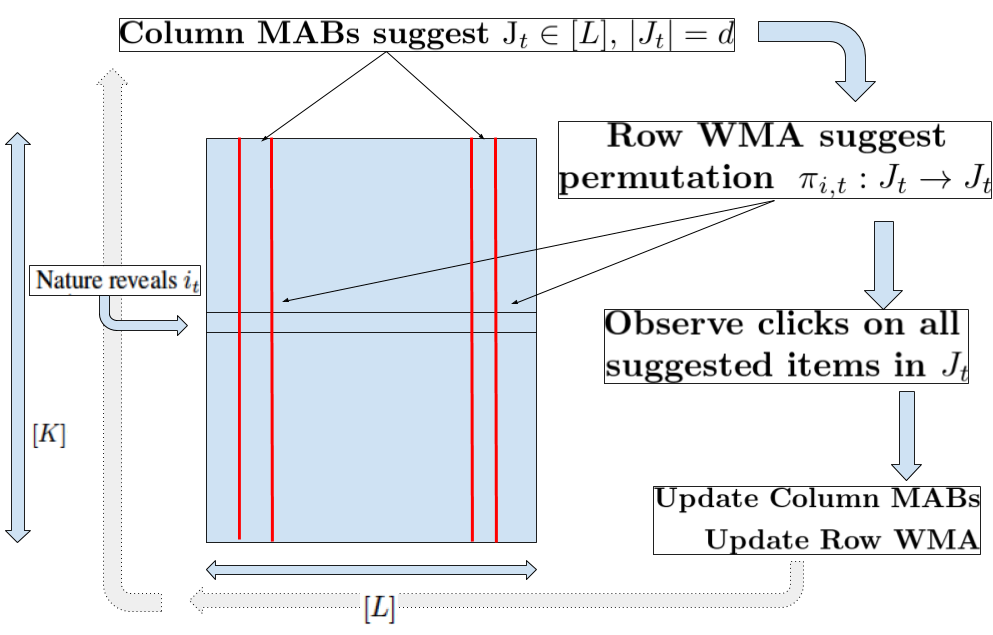
\includegraphics[scale=0.2]{img/RankedBand.png}
%    \caption{Latent Ranked Bandit in rank $d=2$ scenario. \todob{The figure is super confusing. If you want to have it, add a flow chart.}}
%    \label{fig:rankedbandit}
%    \vspace*{-1em}
%\end{figure}

\begin{algorithm}[t]
  \caption{Latent Ranker Algorithm ($\latentranker$)}
  \label{alg:latent ranker}
  \begin{algorithmic}[1]
    \State \textbf{Input:} Rank $d$, horizon $n$
    \State
    \For{$k = 1, \dots, d$}
    \Comment{Initialization}
      \State Initialize $\colalg(k)$
    \EndFor
    \ForAll{$i \in [K], J \subset [L] \text{ such that } |J| = d$}
      \State Initialize $\rowalg(i, J)$
    \EndFor
    \State
    \For{$t = 1, \dots, n$}
      \State User $i_t$ is revealed
      \For{$k = 1, \dots, d$}
      \Comment{Generate response}
        \State $\hat{\ell}_k \gets \text{ Suggested item by } \colalg(k)$
        \If{$\hat{\ell}_k \in \{\ell_1, \dots, \ell_{k - 1}\}$}
          \State $\ell_k \gets$ Random item not in $\{\ell_1, \dots, \ell_{k - 1}\}$
        \Else
          \State $\ell_k \gets \hat{\ell}_k$
        \EndIf
      \EndFor
      \State $J_t \gets (\ell_1, \dots, \ell_d)$
      \State $\pi_{t, i_t} \gets \text{ Suggested permutation by } \rowalg(i_t, J_t)$
      \State
      \State Recommend $\pi_{t, i_t}(J_t)$
      \State Observe $M_t(i_t, J_t(k))$ for all $k \in [d]$
      \State
      \For{$k = 1, \dots, d$}
      \Comment{Update statistics}
        \If{$\ell_k = \hat{\ell}_k$}
          \State Update arm $\ell_k$ of $\colalg(k)$ with reward
          \begin{align*}
            \qquad \quad & \max \, \{M_t(i_t, J_t(a)): a \in [k]\} - {} \\
            & \max \, \{M_t(i_t, J_t(a)): a \in [k - 1]\}
          \end{align*}
        \Else
          \State Update arm $\hat{\ell}_k$ of $\colalg(k)$ with reward $0$
        \EndIf
      \EndFor
      \ForAll{arms $\pi$ in $\rowalg(i_t, J_t)$}
        \State Update arm $\pi$ with reward $r_t(i_t, \pi(J_t))$ in \eqref{eq:reward}
      \EndFor
    \EndFor
  \end{algorithmic}
\end{algorithm}


\subsection{Practical Considerations}
\label{sec:practical considerations}

\todob{Discuss time and space complexities of $\latentranker$.}

\todob{Say how we hack $\rowalg$.}

\todob{Discuss suitable choices for $\colalg$ and $\rowalg$.}


\section{Experiments}
\label{sec:experiments}
In this section, we compare $\latentranker$ to several bandit algorithms in three experiments. The first two experiments are on synthetic dataset where all modeling assumptions hold. The third experiment is on a real-life dataset where we evaluate $\latentranker$ when our modeling assumptions fail. All results are averaged over $10$ independent random runs. We test in both rank $1$ and rank $2$ settings to clearly illustrate the failures of the current Rank-$1$ algorithms and show the efficiency of our proposed method. We use the term rows/users and columns/items interchangeably.
%In all our experiments user come uniform randomly over all time $[n]$. 

\subsection{Evaluated Algorithms}

\textbf{Rank $1$ Algorithms:} We compare against several state-of-the-art rank $1$ algorithms. Note, that all the rank $1$ algorithms suggest a single row and column at every round. The $\ucb$ algorithm from \citet{auer2002finite} builds a confidence set at every round $t$ over all the entries of $M_t$ as $c_{i, j}(t) = \sqrt{\frac{2\log t}{N_{i, j}(t)}}$ where $N_{i, j}(t)$ denotes the number of times the $M(i,j)$-th entry has been observed. It the suggests the best row-column pair based on the term $\hat{M}_{t}(i,j) + c_{i, j}(t)$ where $\hat{M}_{t}(i,j)$ denotes the empirical mean of all the observed rewards for $M(i,j)$. The $\ucbe$ \citep{auer2010ucb} is similar to $\ucb$ but it eliminates sub-optimal rows and columns  based on a similar confidence set  $c_{i, j}(t)$ till it finally converges on the best pair of row and column. The algorithm $\linucb$ was first proposed in \citet{li2010contextual} for the contextual bandit setting. Note, that for a set of features $\theta \in {0,1}^{K+L}$, rank-$1$ bandit generalizes to the stochastic linear bandit setting and can be solved by $\linucb$. Similarly, GLM-UCB from  \citet{filippi2010parametric} which computes the maximum-likelihood estimates of the parameter vector $\theta \in {0,1}^{K+L}$ (using Expectation-Maximization algorithm) can also be used solve the rank $1$ bandit problem. Finally, we compare against the algorithm $\rankelim$ from \citet{katariya2016stochastic} which is an improved version of $\ucbe$ and employs row and column elimination and aggressive exploration to converge on the best row and column pair. For $\latentranker$ we use the Algorithm \ref{alg:LRB} from Section \ref{sec:rank1}. 
%We use \expthree as the \rowalg and \colalg with the exploration parameter $\gamma_{\text{\rowalg}} = \sqrt{\frac{K\log K}{T}}$ and $\gamma_{\text{\colalg}} = \sqrt{\frac{L\log L}{T}}$ respectively.


\textbf{Rank $2$ Algorithms:} We similarly design the Rank $2$ algorithms by modifying the rank $1$ algorithms. Again, note that all the rank $2$ algorithms suggest two pairs of rows and columns at every round $t$. For all of the algorithms $\ucb$, $\ucbe$, $\linucb$, $\glmucb$, and $\rankelim$ we modify these algorithms so that they suggest $2$ pairs of rows and columns based on their respective confidence interval set $c_{i, j}(t)$. The row and column pair with the highest and the second highest $\hat{M}_{t}(i,j) + c_{i, j}(t)$ are suggested for each round $t$ and consequently after observing all the entries of $M_t(i,j)$ all of the algorithms update their estimates of $\hat{M}_{t}(i,j)$ for each $i,j \in [d]$. For $\latentranker$ we use the Algorithm \ref{alg:LRB1} from Section \ref{sec:algorithm}. Note, that there are two $\rowalg$ and $\colalg$, each running an $\expthree$ algorithm with the  exploration parameters as discussed before. For $\latentranker$ we use the Algorithm \ref{alg:LRB1} from Section \ref{sec:algorithm}. 

\subsection{Synthetic Experiment $1$}
This experiment is conducted to test the performance of $\latentranker$ over a small number of users and items and to show how $\latentranker$ scales with increasing number of users and items. Note, that in this experiment all our modeling assumptions hold. This simulated testbed consist of two scenarios: (1) $8$ users and $8$ items and (2) $16$ users and $16$ items. In this setting, $U = \{0.7, 0.9\}^{K\times 1}$ and similarly $V = \{0.7, 0.9\}^{L\times 1}$ with the entry $U(K/2,1) = V(L/2,1) = 0.9$. Hence, the matrix $M = UV^{\intercal}$ is rank $1$ and the hott-topics structure is maintained. At every round $t$, $u_t(i)$ is an independent Bernoulli variable with mean $U(i,1)$ and $v_t(j)$ is an independent Bernoulli variable with mean $v_t(j) = V(j,1)$. The learner observes the entry $u_t(i)v_t(j)$ when it selects the $i$-th user and $j$-th item. A similar environment has been discussed as $B_{\text{spike}}$ in \citep{katariya2016stochastic}. From Figure \ref{fig:2} we can clearly see that $\latentranker$ outperforms all the other algorithms. The regret curve of $\latentranker$ flattens, indicating that it has learned the best user-item pair. As we scale the number of users and items we see that $\latentranker$ performs even better than other algorithms. The key realization is that $\latentranker$ takes advantage of the hott-topics structure and quickly identifies them. Note, that for any rank $d$ scenario the best user-item pair must be one of the hott-topics in $(I^*, J^*)$.

%$u_t = \mathcal{D} + \Delta_u$ and $v_t =  \mathcal{D}_t  + \Delta_v$, where $\mathcal{D}_t \in \{0,1\}$ is independent Bernoulli noise and $\Delta_u = \Delta_v = 0.2$
%Independent user model algorithms $\RBAUCB$ and $\RBAEXP$  perform poorly as the number of items per user is too large and the independent algorithms are not sharing information between them. $\NMFBan$ performs better than the independent user model algorithms but is outperformed by $\LRAEXP$, $\LRATS$ and $\LRAUCB$.


%The vectors spanning $U$ and $V$, generating the user-item preference matrix $M$, are shown Figure \ref{fig:1}. The users are evenly distributed into a $50:50$ split such that $50\%$ of users prefer item $1$ and $50\%$ users prefer item  $2$. The item hott-topics are $V(1,:) = (0,1)$ and $V(2,:) = (1, 0)$ while remaining $70\%$ of items has feature $V(j',:) = (0.45, 0.55)$ and the rest have $V(j,:) = (0.55, 0.45)$. We create the user feature matrix $U$ similarly having a $50:50$ split such that $U(1,:) = (0,1)$, $U(2,:) = (0.2,0.8)$ and the remaining $70\%$ users having $U(i,:) = (0,0.8)$ and $30\%$ users having $U(i',:) = (0.7,0)$. At every timestep $t$ the resulting matrix $M_t =UD_tV^{\intercal}$ is generated where $D_t$ is a randomly-generated diagonal matrix. So, $M_t$ is  such that algorithms that quickly find the easily identifiable hott-topics perform very well. From Figure \ref{fig:2} we can clearly see that $\LRAEXP$, $\LRATS$ and $\LRAUCB$ outperforms all the other algorithms. Their regret curve flattens, indicating that they have learned the best items for each user. Independent user model algorithms $\RBAUCB$ and $\RBAEXP$  perform poorly as the number of items per user is too large and the independent algorithms are not sharing information between them. $\NMFBan$ performs better than the independent user model algorithms but is outperformed by $\LRAEXP$, $\LRATS$ and $\LRAUCB$.

\subsection{Synthetic Experiment $2$}
This experiment is conducted to test the performance of $\latentranker$ over a large number of users and items. This simulated testbed consist of $64$ users, $64$ items, and rank$(M) = 2$. The vectors spanning $U$ and $V$, generating the user-item preference matrix $M$, are shown Figure \ref{fig:3}. The users and items are evenly distributed into a $50:50$ split such that $50\%$ of users prefer item $1$ and $50\%$ users prefer item $2$. The item hott-topics are $V(1,:) = (1,0)$ and $V(2,:) = (0, 0.6)$ while $50\%$ remaining  items has feature $V(j',:) = (0.45, 0.5)$ and the rest have $V(j,:) = (0.5, 0.45)$. Similarly, we create the user feature matrix $U$ having a $50:50$ split such that $U(1,:) = (1,0)$, $U(2,:) = (0,0.6)$ and the remaining $50\%$ users having $U(i,:) = (0.5,0.4)$ and the rest having $U(i',:) = (0.4,0.5)$. At every timestep $t$ the resulting matrix $M_t =UD_tV^{\intercal}$ is generated where $D_t$ is a randomly-generated diagonal matrix. So, $M_t$ is such that algorithms that quickly find the easily identifiable hott-topics perform very well. From Figure \ref{fig:2} we can clearly see that $\latentranker$ outperforms all the other algorithms. It's  regret curve flattens, indicating that it has learned the best user-item pair. 

%Independent user model algorithms $\RBAUCB$ and $\RBAEXP$  perform poorly as the number of items per user is too large and the independent algorithms are not sharing information between them. $\NMFBan$ performs better than the independent user model algorithms but is outperformed by $\LRAEXP$, $\LRATS$ and $\LRAUCB$.



\begin{figure}[!th]
\centering
\begin{tabular}{cc}
\setlength{\tabcolsep}{0.1pt}
\subfigure[0.25\textwidth][Expt-$1$: $8$ Users, $8$ items, Rank $1$, Algorithm Performance]
    %with $r_{i_{{i}\neq {*}}}=0.07$ and $r^{*}=0.1$
    {
    		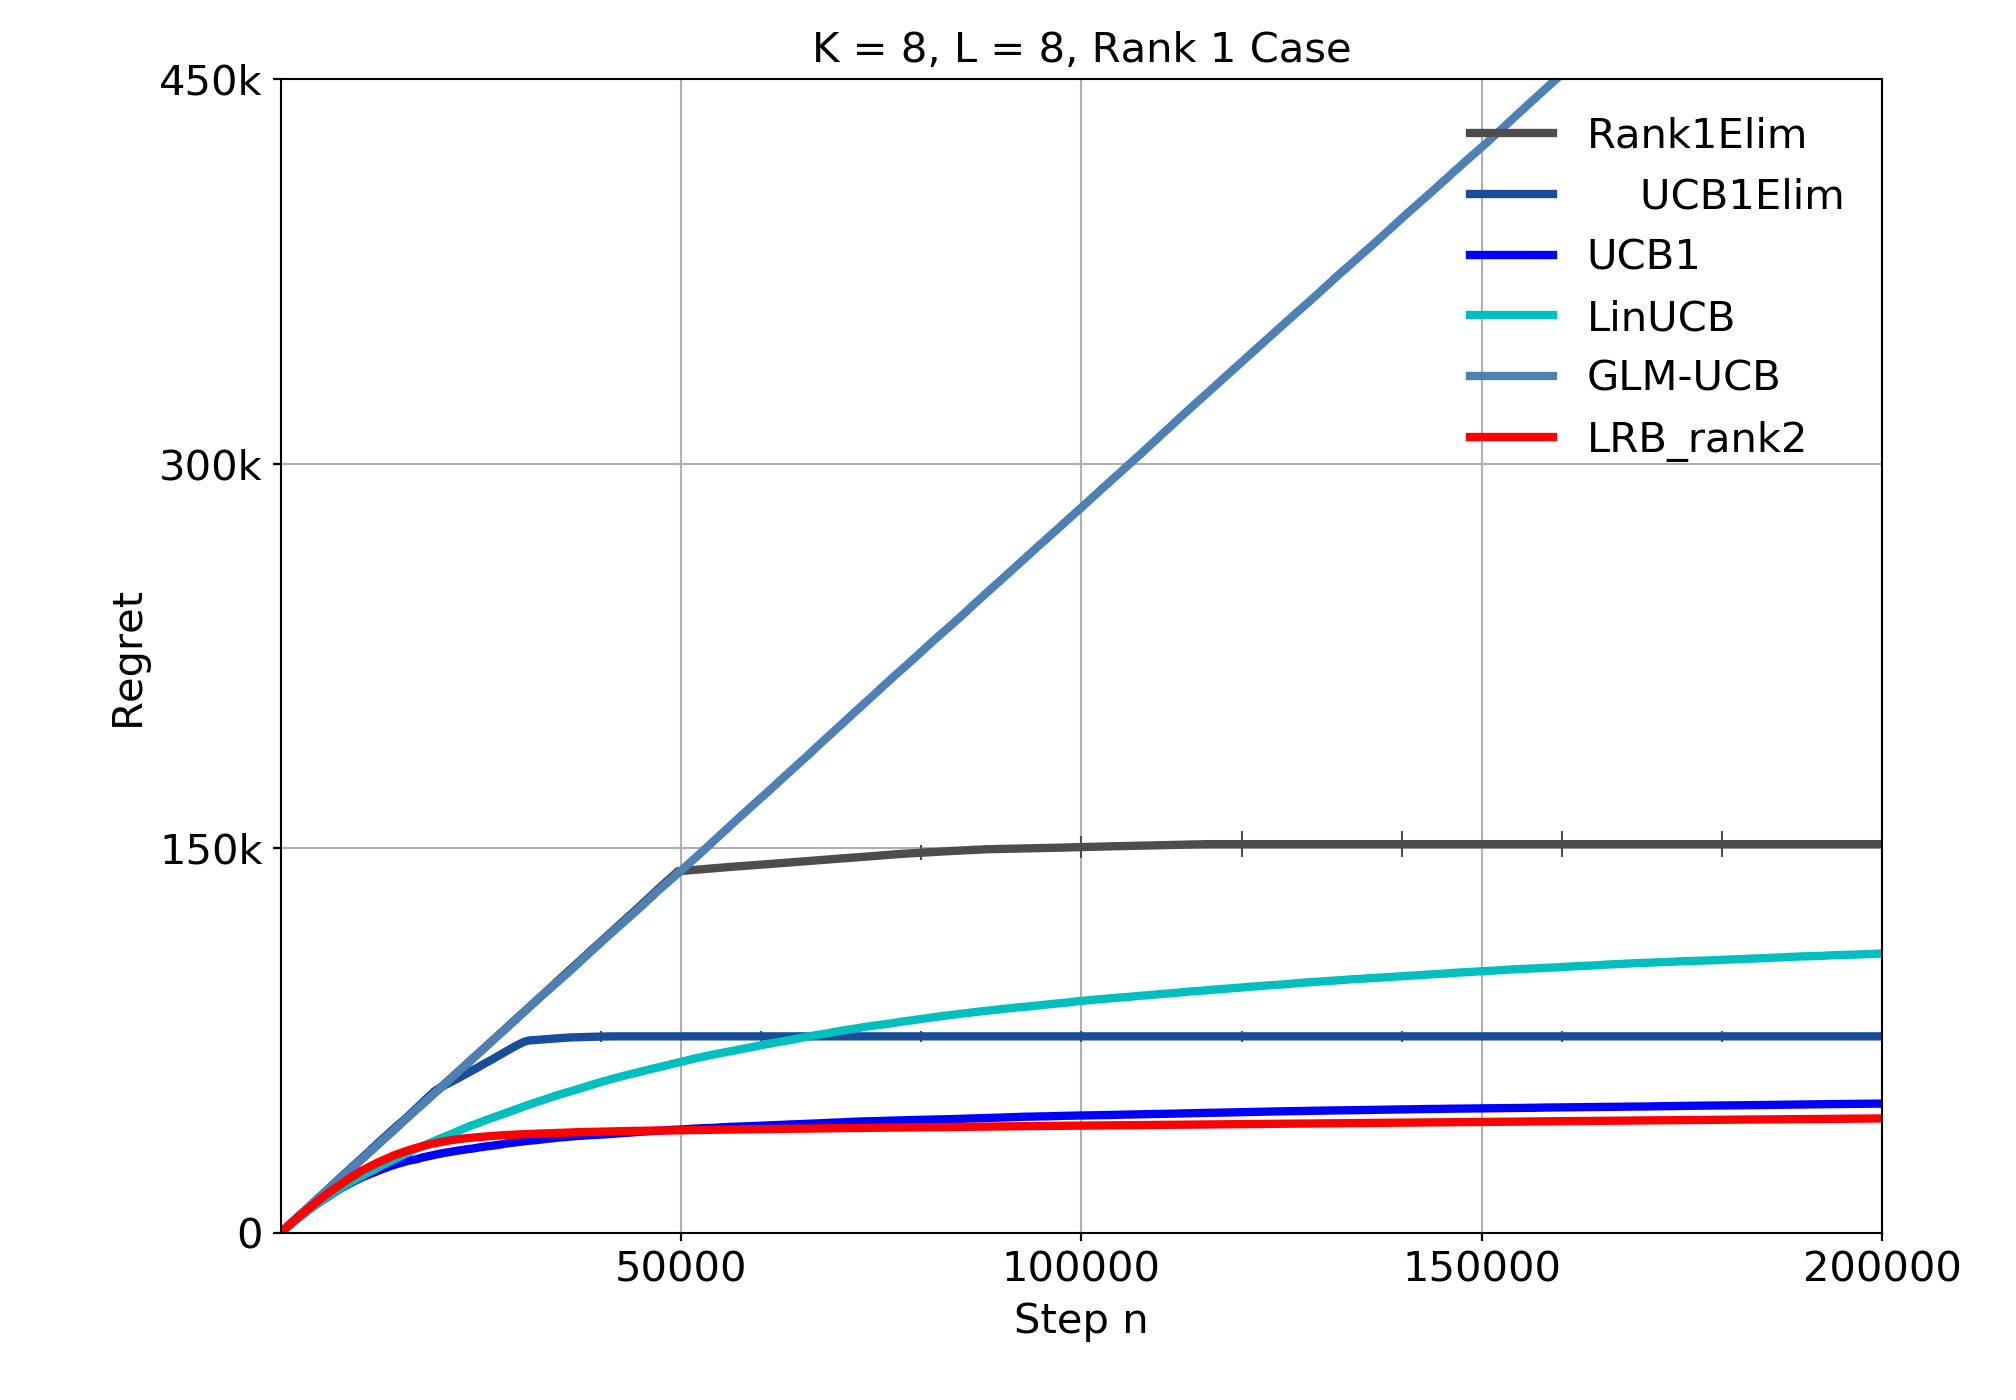
\includegraphics[scale=0.13]{img/Figure_8.png}
  		\label{fig:1}
    }
    &
    \subfigure[0.25\textwidth][Expt-$1$: $16$ Users, $16$ items, Rank $1$, Algorithm Performance]
    %with $r_{i_{{i}\neq {*}}}=0.07$ and $r^{*}=0.1$
    {
    		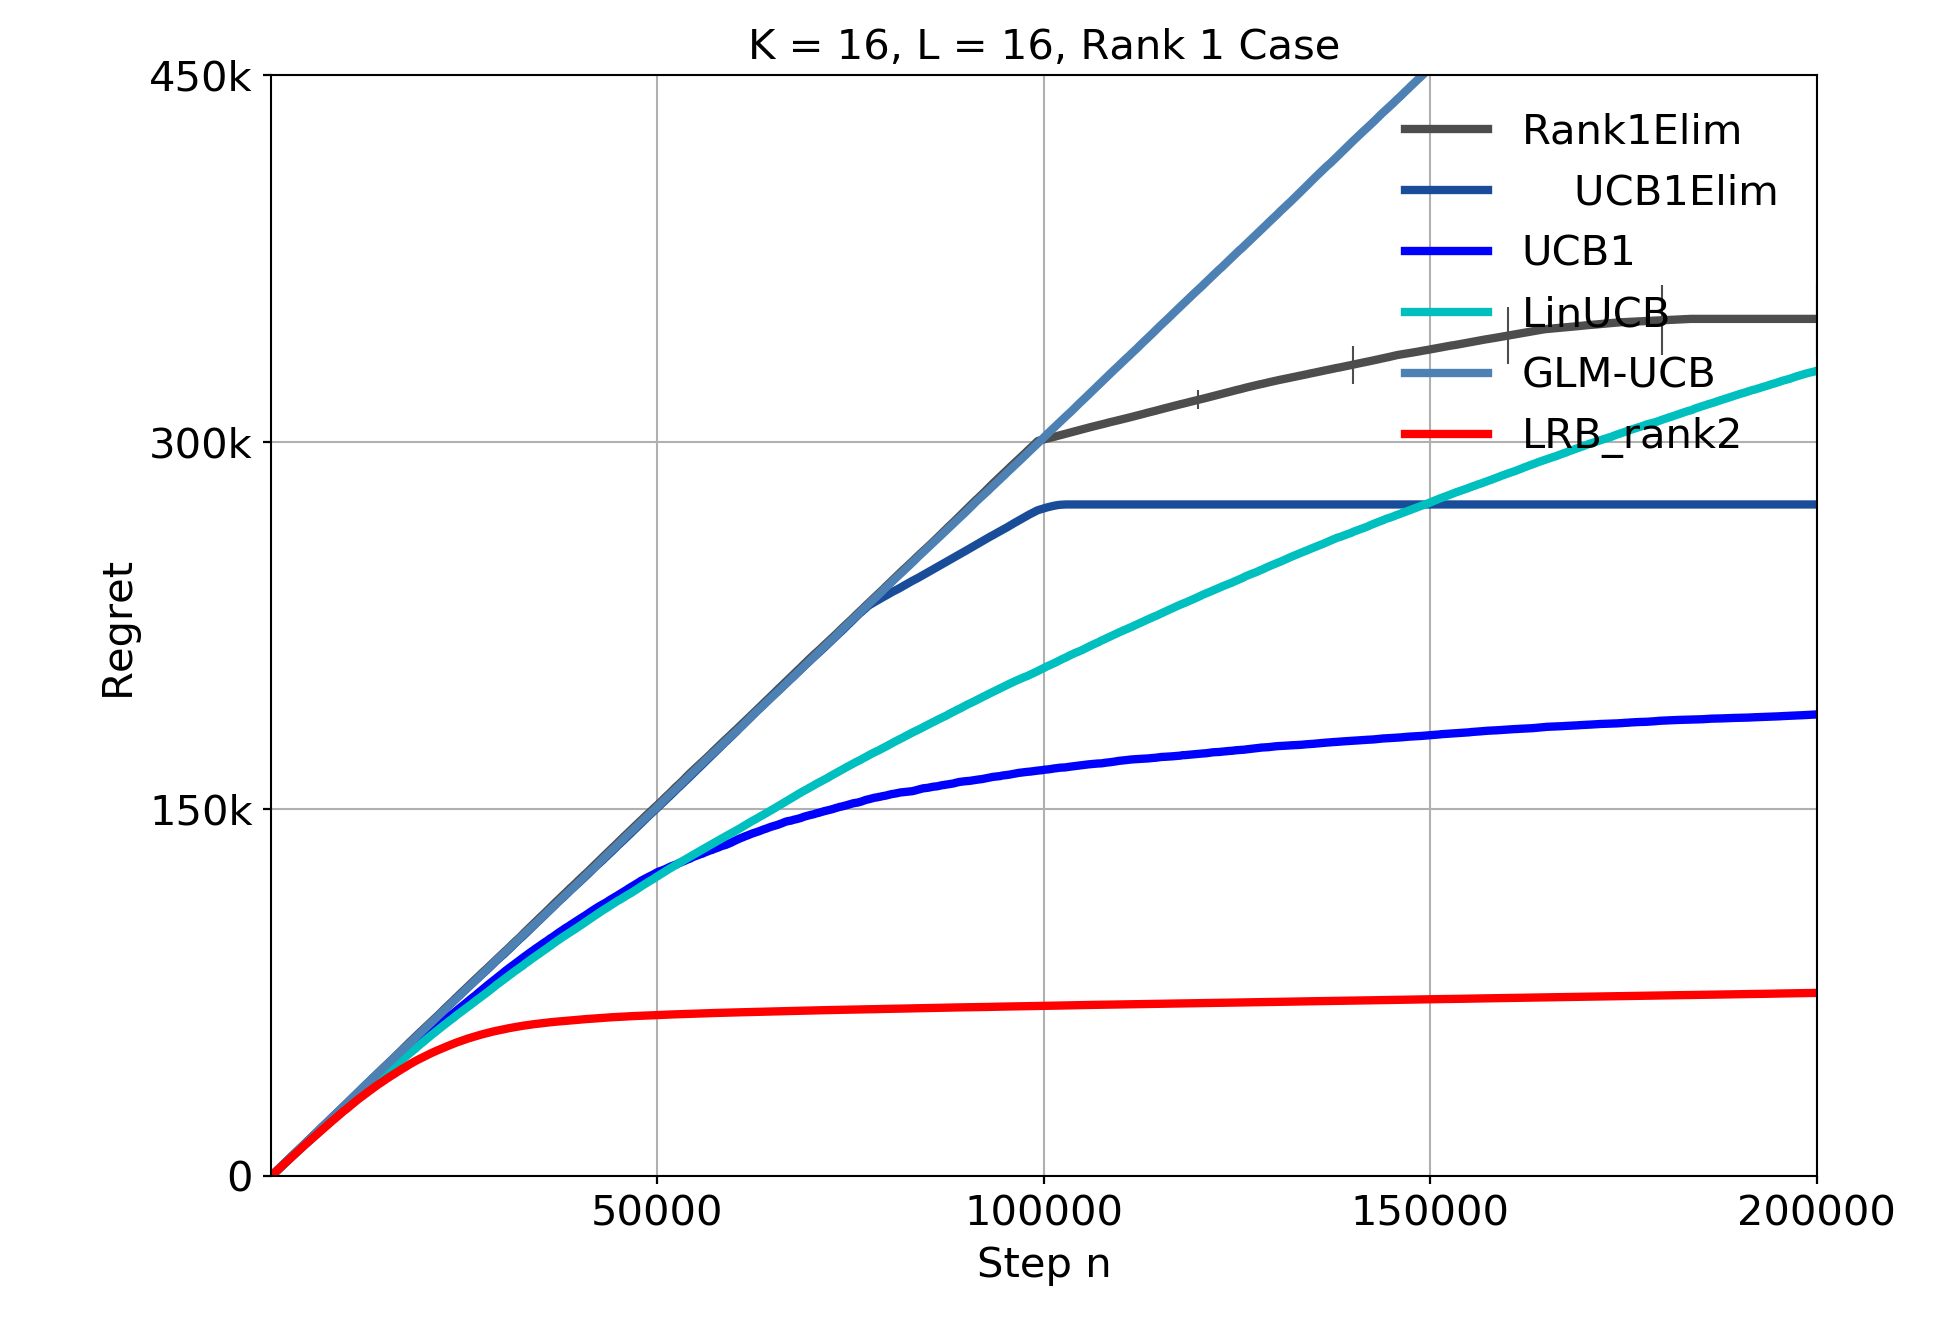
\includegraphics[scale=0.13]{img/Figure_16.png}
  		\label{fig:2}
    }
    \\
    \subfigure[0.25\textwidth][Expt-$2$: $64$ Users, $64$ items, Rank $2$, User and Item vectors]
    %with $r_{i_{{i}\neq {*}}}=0.07$ and $r^{*}=0.1$
    {
    		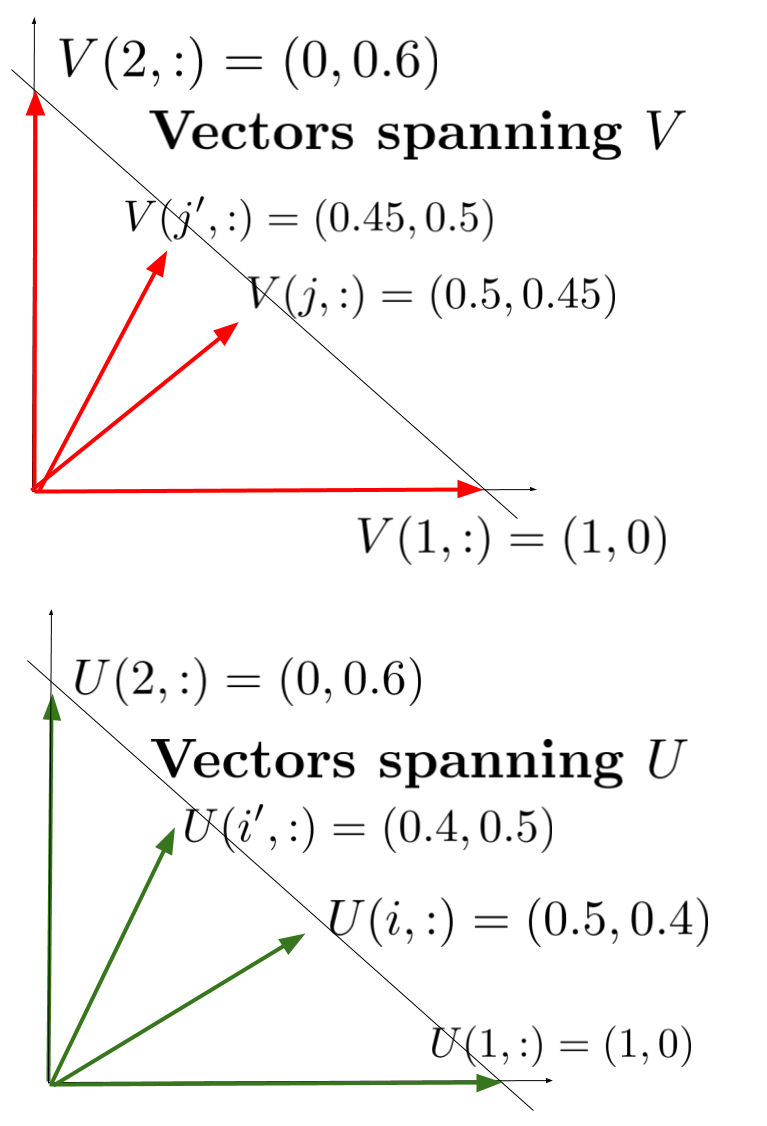
\includegraphics[scale=0.08]{img/rank_21_vec.png}
  		\label{fig:3}
    }
    &
    \subfigure[0.25\textwidth][Expt-$2$: $64$ Users, $64$ items, Rank $2$, Algorithm Performance]
    %with $r_{i_{{i}\neq {*}}}=0.07$ and $r^{*}=0.1$
    {
    		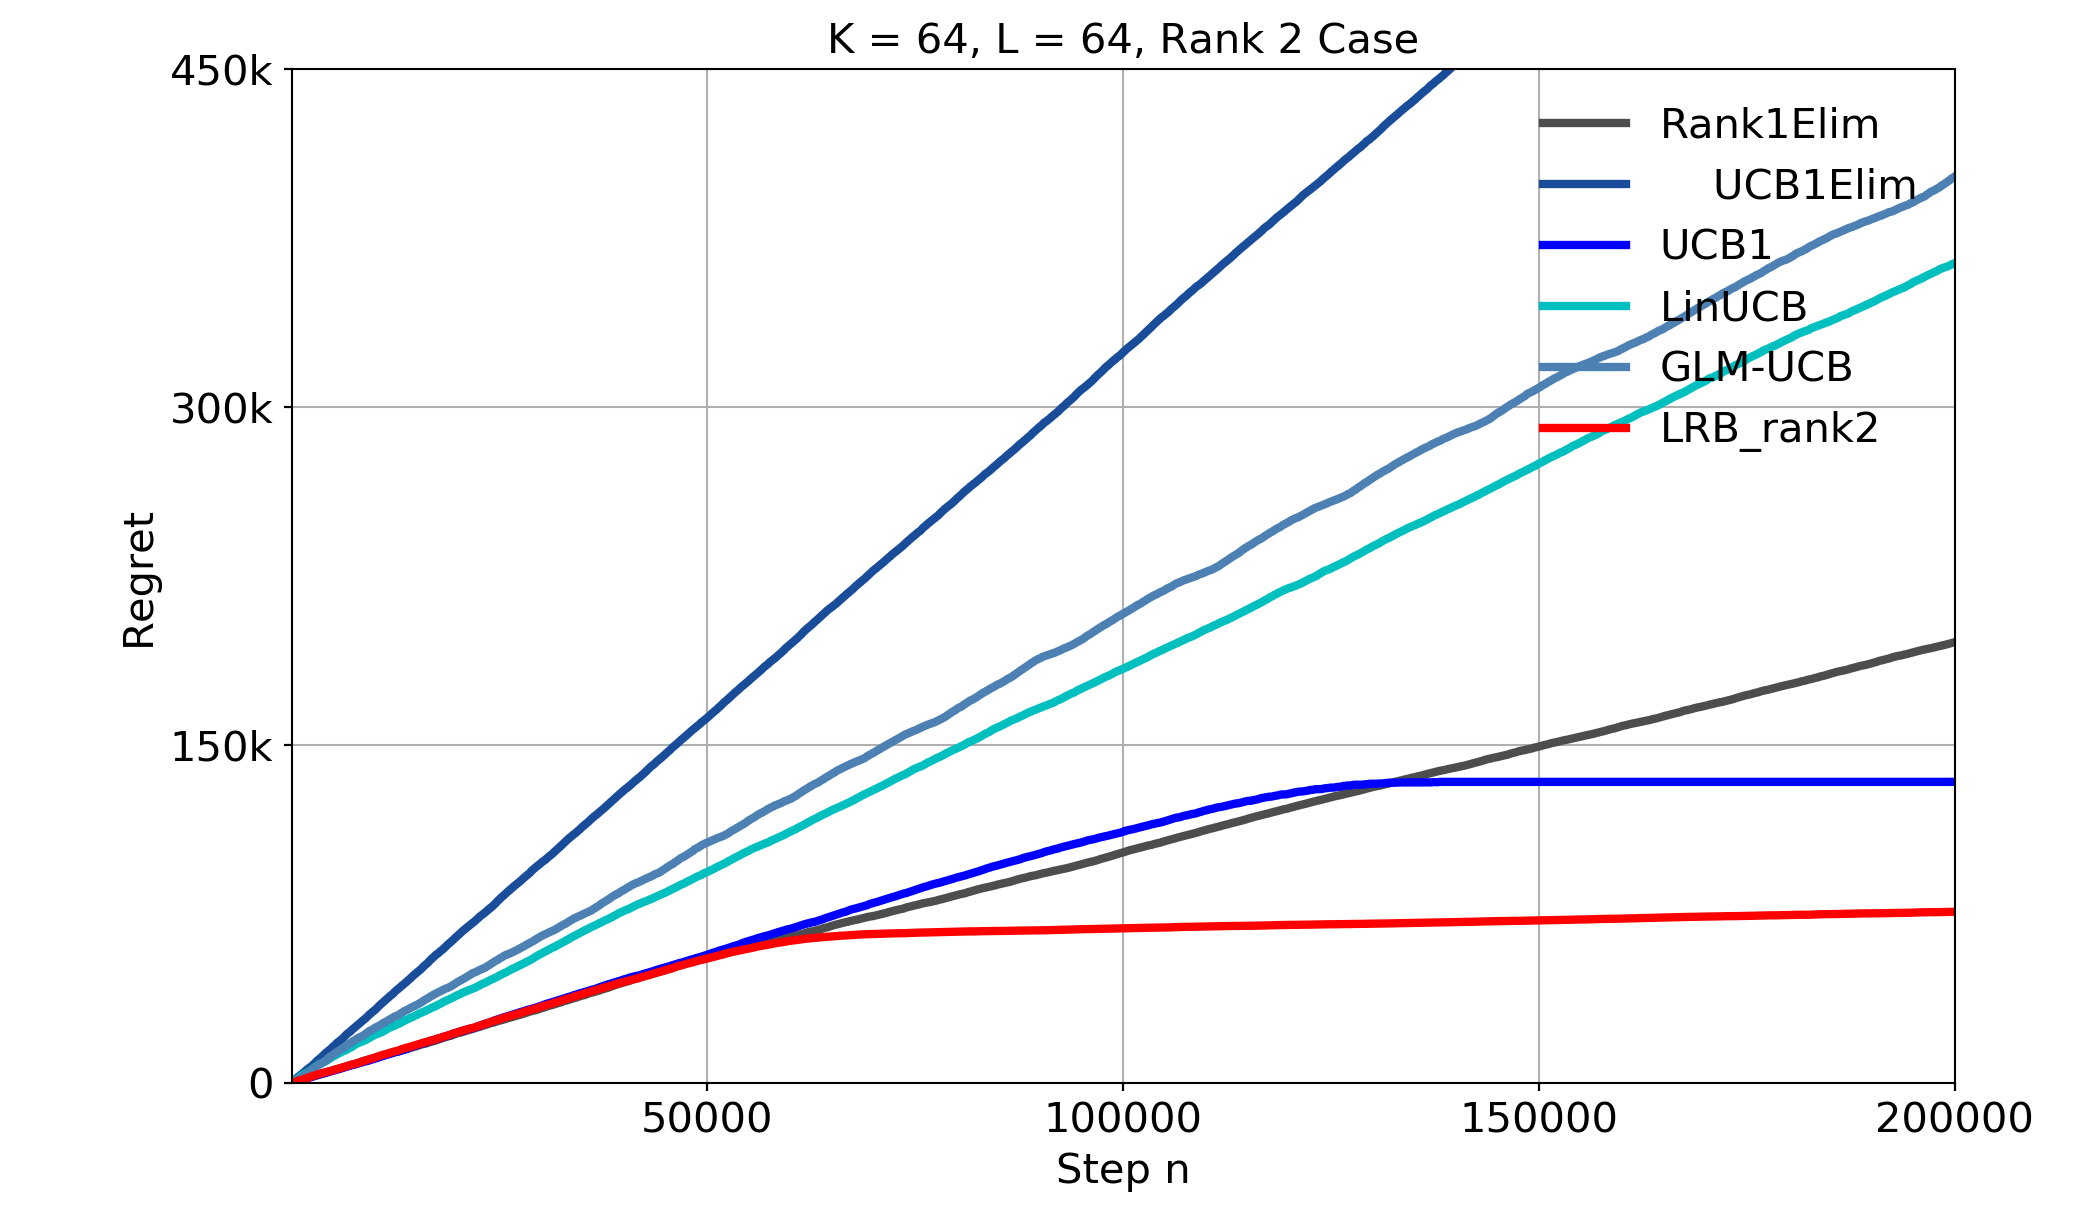
\includegraphics[scale=0.13]{img/Figure_64.png}
  		\label{fig:4}
    }
    \end{tabular}
    \caption{A comparison of the cumulative regret incurred by the various bandit algorithms. }
    \label{fig:karmed1}
    \vspace*{-1em}
\end{figure}


\subsection{Real World Experiment $3$}
We conduct the third experiment to test the performance of \latentranker when our modeling assumptions are violated. We use the Jester dataset \citep{goldberg2001eigentaste} which consist of over 4.1 million continuous ratings of 100 jokes from 73,421 users collected over 5 years. In this dataset there are many users who rated all jokes and we work with these users. Hence the user-item preference matrix is fully observed and we will not have to complete it using matrix completion techniques. Hence, this approach is very real world. We sample randomly $10$ users (who have rated all jokes) from this dataset and use singular value decomposition (SVD) to obtain a rank $2$ approximation of this user-joke rating matrix $M$. In the resultant matrix $M$, most of the users belong to the two classes preferring jokes $98$, and $28$, while a very small percentage of users prefer some other jokes. Note, that this condition results from the fact that this real-life dataset does not have the hott-topics structure. Furthermore, in this experiment we assume that the noise is independent Bernoulli over the entries of $M$ and hence this experiment deviates from our modeling assumptions. From \ref{fig:6} again we see that $\latentranker$ outperform other algorithms. 
\begin{wrapfigure}{l}{0.2\textwidth}
 \subfigure[0.2\textwidth][Expt-$3$: $10$ Users, $100$ items, Rank $2$, Jester Dataset]
    %with $r_{i_{{i}\neq {*}}}=0.07$ and $r^{*}=0.1$
    {
    		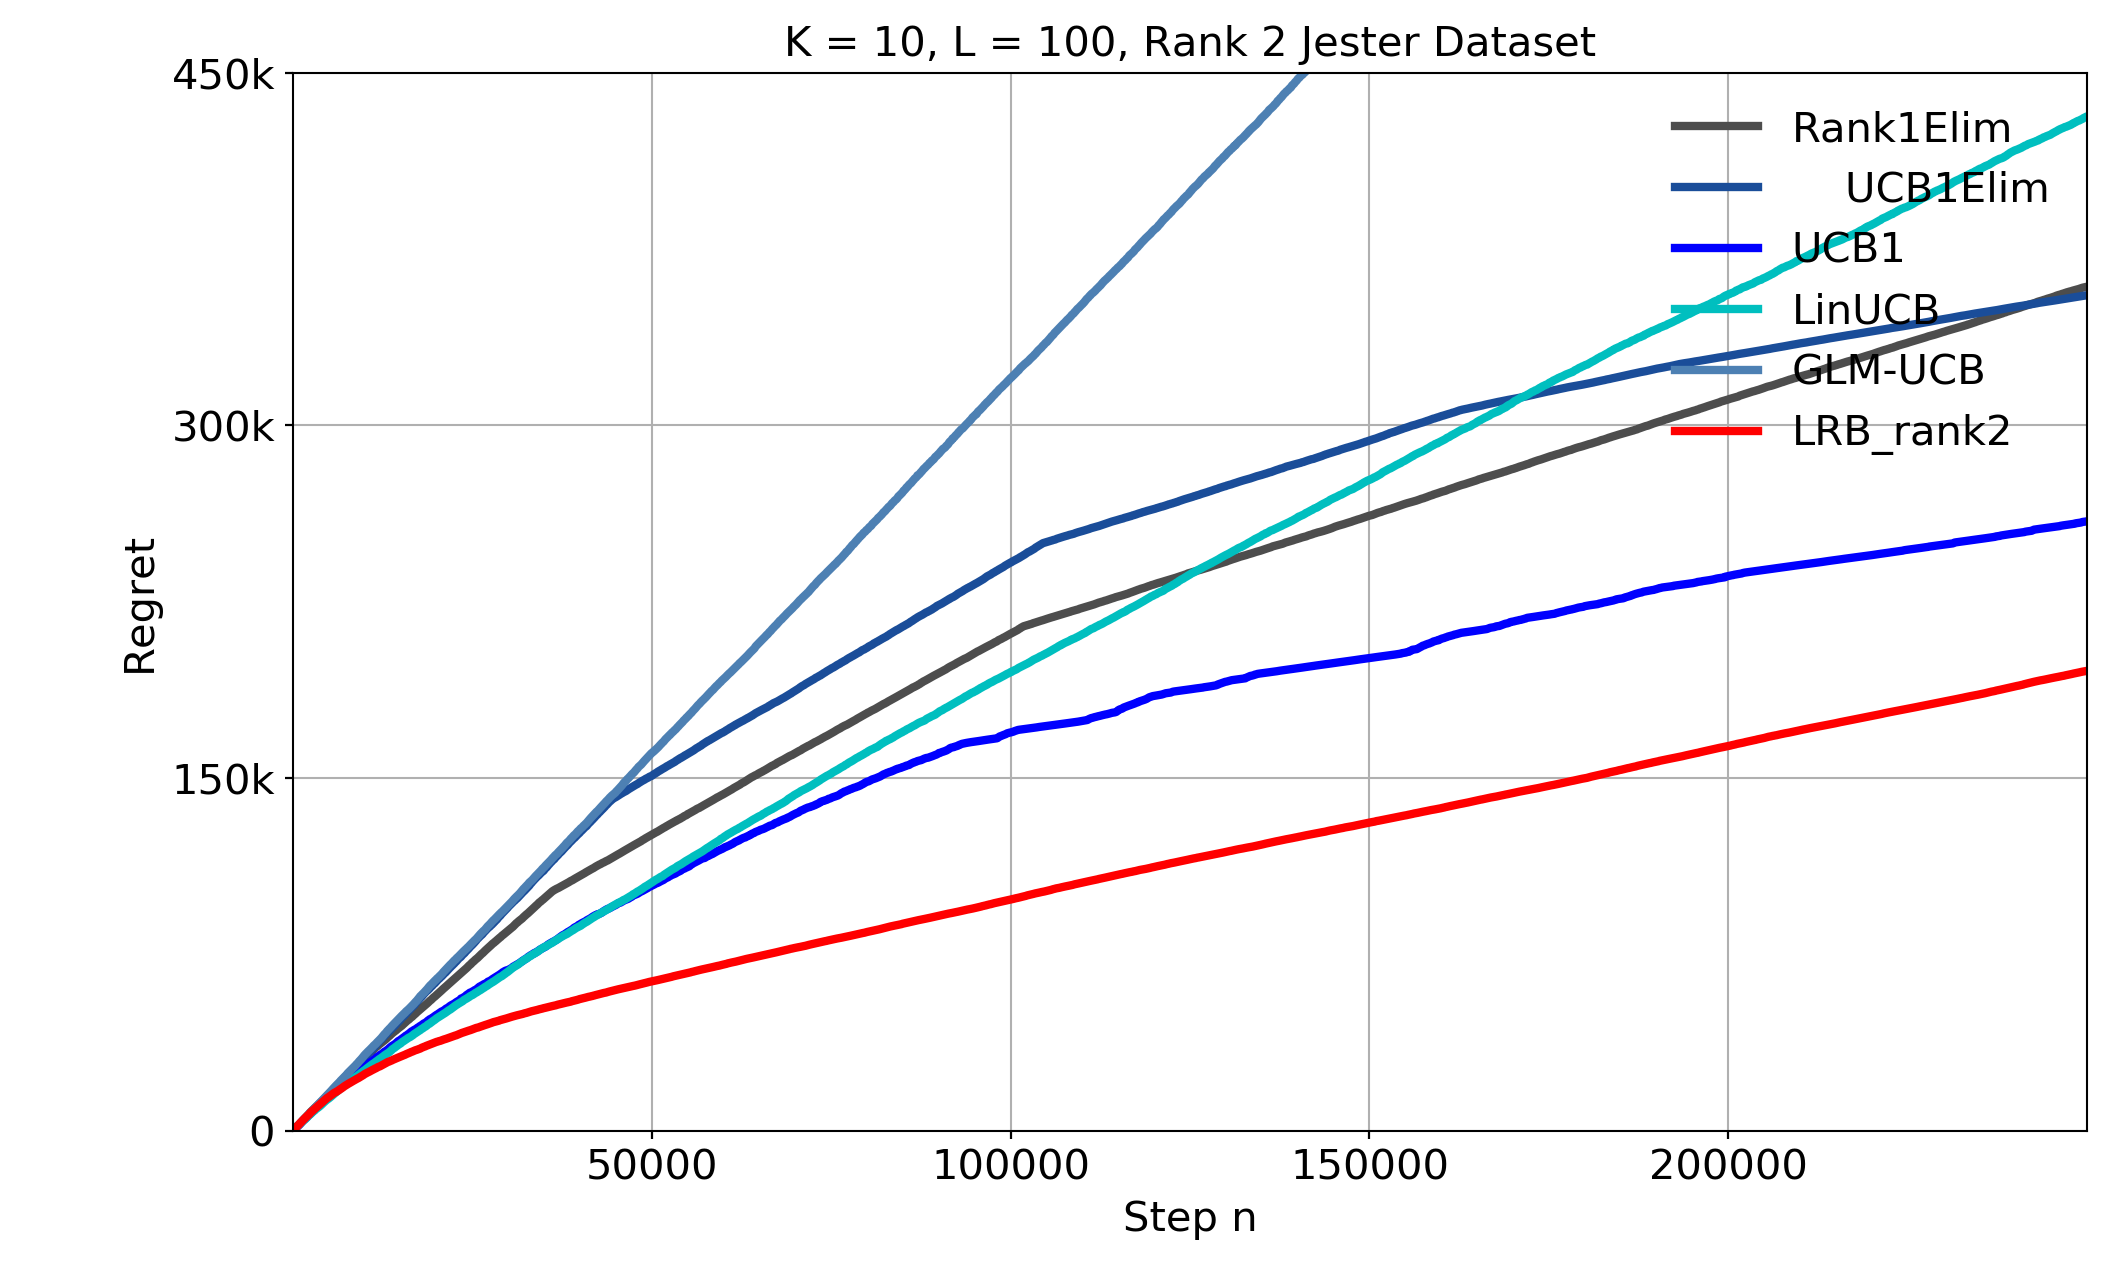
\includegraphics[scale=0.13]{img/Figure_J_1.png}
  		\label{fig:6}
    }
\end{wrapfigure}

%The rank $2$ approximation of $M$ of  is shown in Figure \ref{fig:5}, where we can clearly see the red stripes spanning the matrix indicating the low-rank structure of $M$. 
%\begin{figure}[!th]
%\centering
%\begin{tabular}{cc}
%\setlength{\tabcolsep}{0.1pt}
%\subfigure[0.25\textwidth][Expt-$1$: $500$ Users, $50$ items, Rank $2$, User and Item vectors]
%    %with $r_{i_{{i}\neq {*}}}=0.07$ and $r^{*}=0.1$
%    {
%    		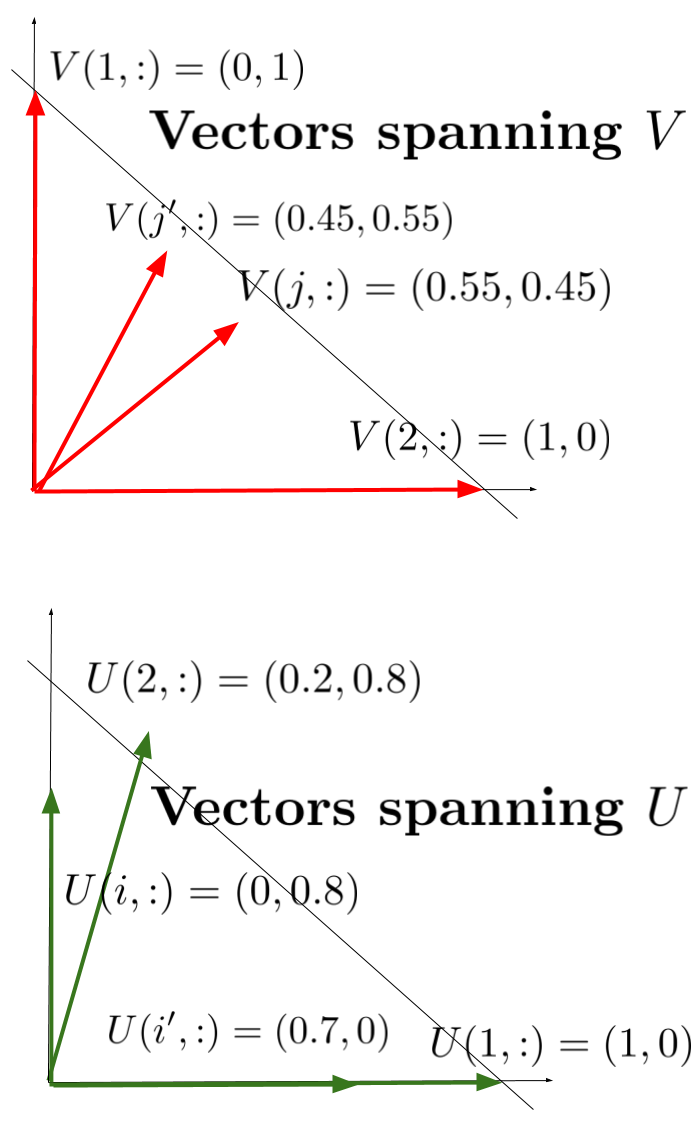
\includegraphics[scale=0.11]{img/rank2_vec.png}
%  		\label{fig:5}
%    }
%    &
%    \subfigure[0.25\textwidth][Expt-$1$: $500$ Users, $50$ items, Rank $2$, User and Item vectors]
%    %with $r_{i_{{i}\neq {*}}}=0.07$ and $r^{*}=0.1$
%    {
%    		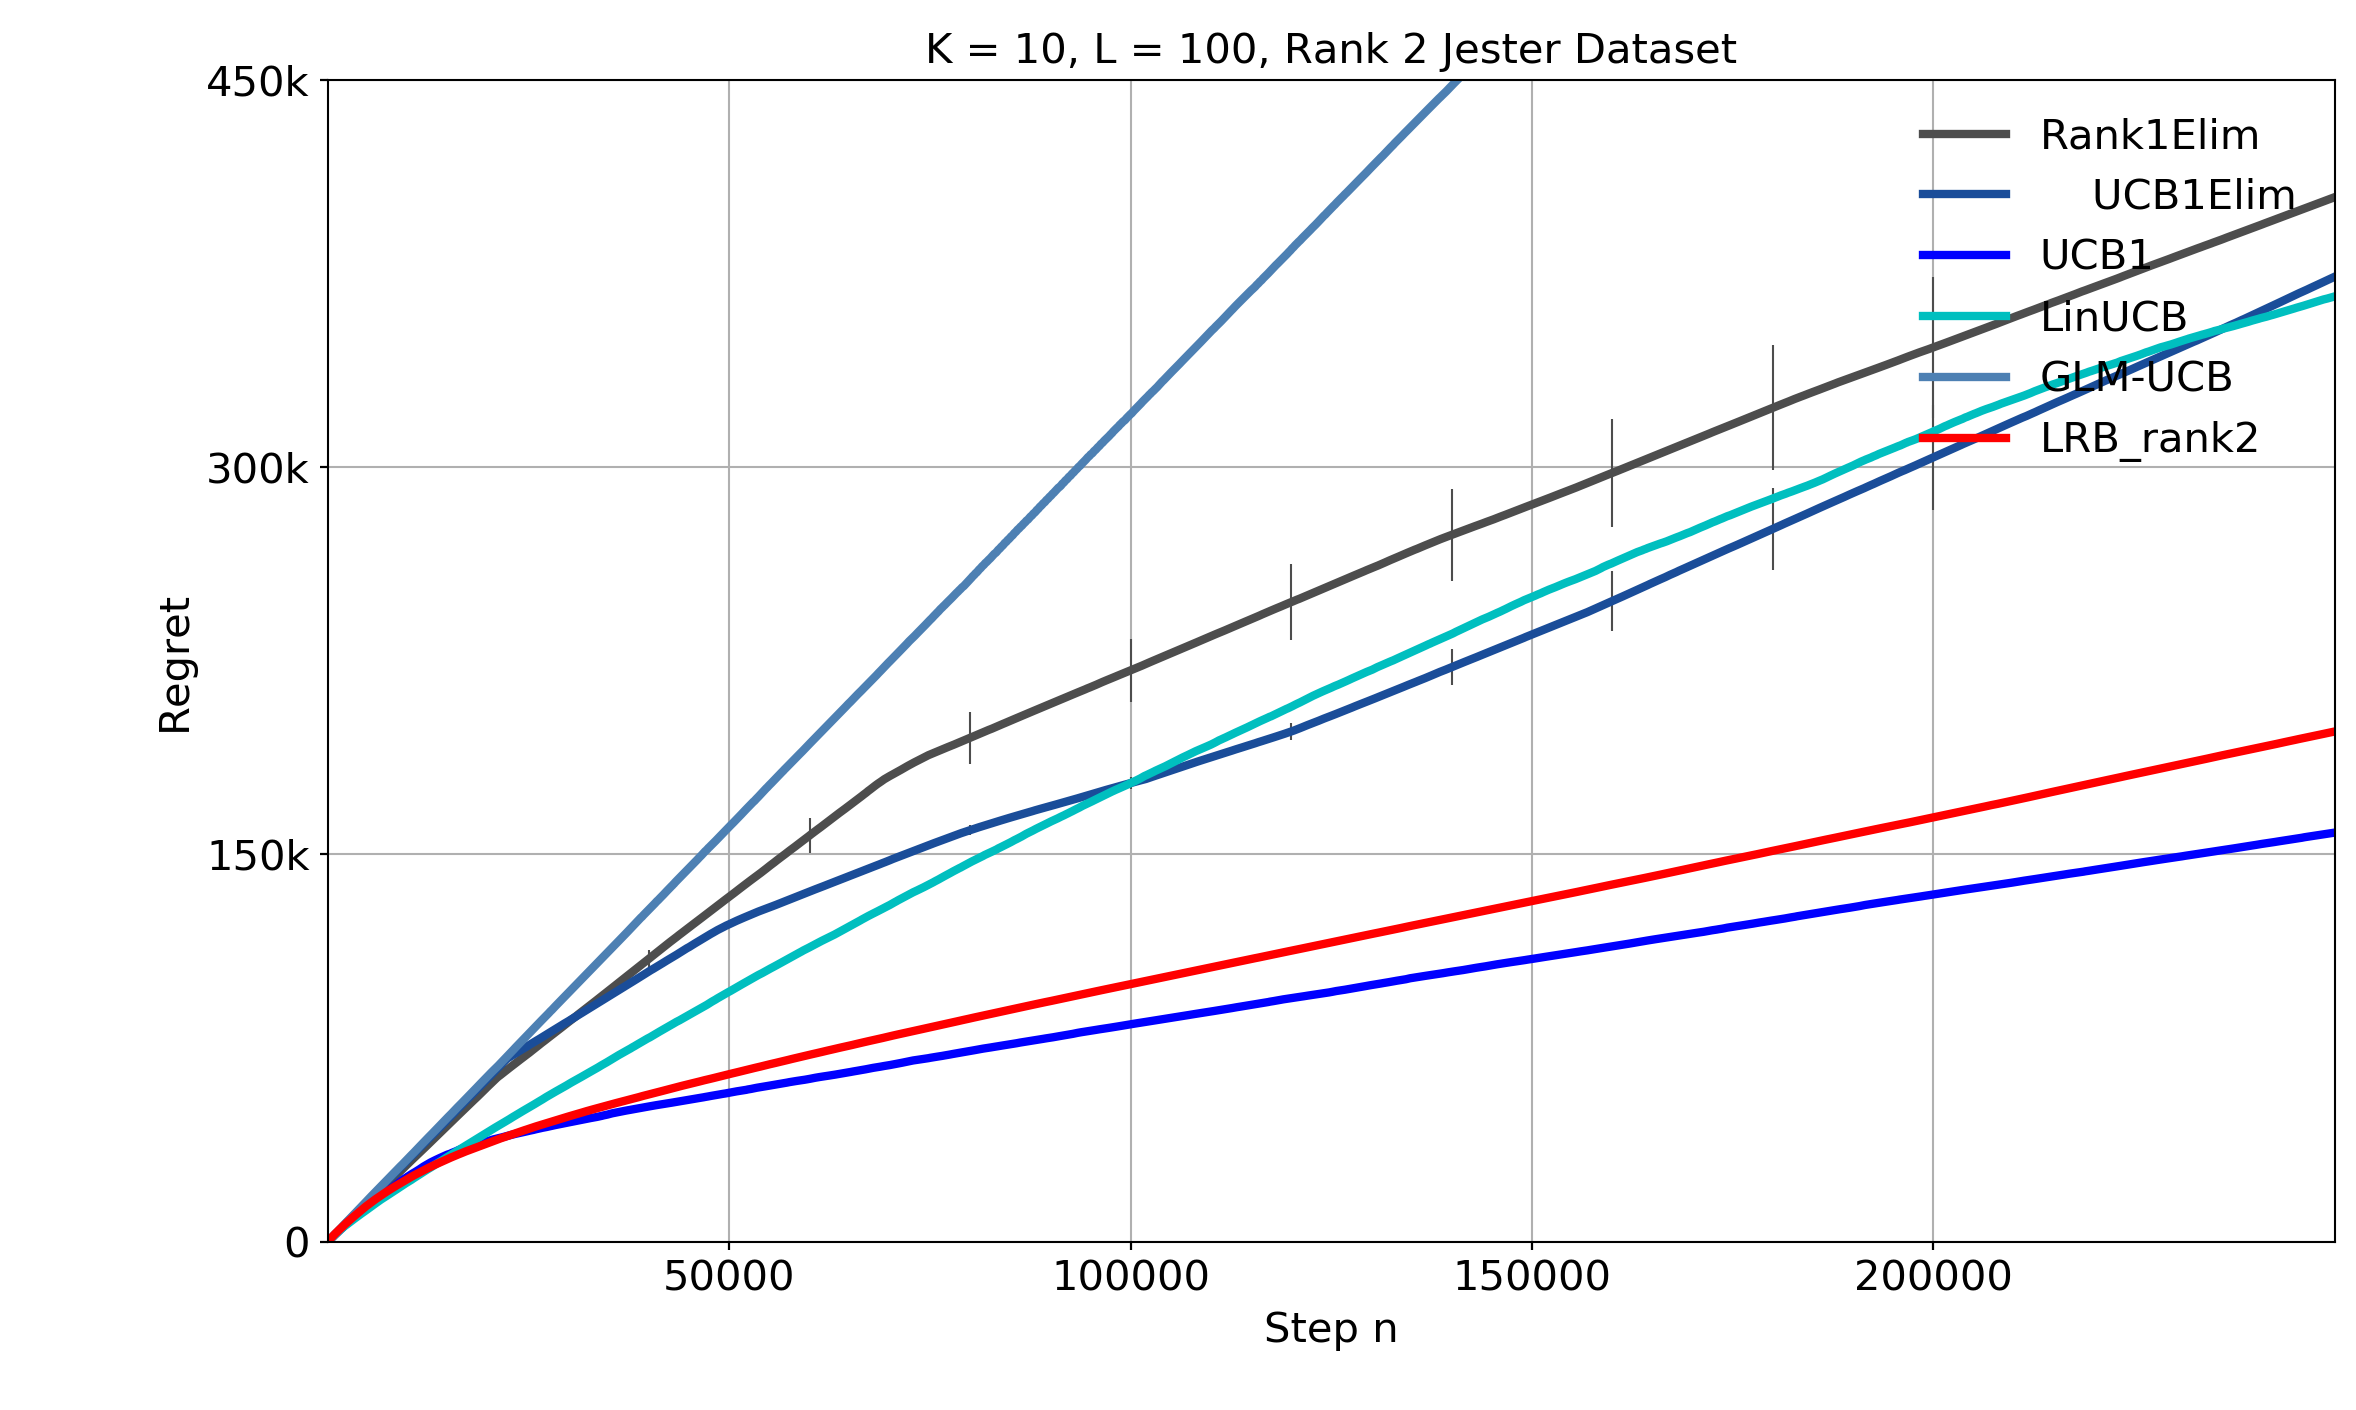
\includegraphics[scale=0.11]{img/Figure_J.png}
%  		\label{fig:1}
%  		\label{fig:6}
%    }
%    \end{tabular}
%    \caption{A comparison of the cumulative regret incurred by the various bandit algorithms. }
%    \label{fig:karmed1}
%    \vspace*{-1em}
%\end{figure}
\vspace*{-1em}
\section{Related Works}
\label{sec:related}
Previous works that have studied this setting have focused either on the rank-$1$ setting or proposed solution where the underlying distributions are stochastic with additional structure.

\textbf{Rank-$1$ Setting:} The work of \citet{katariya2016stochastic} was proposed for a rank-$1$ bandit model with the assumption that the underlying distributions are stochastic. Similarly, \citet{katariya2017bernoulli} was proposed for the special case when the underlying distributions are Bernoulli.  A more simpler setting has also been studied in \citet{maillard2014latent}. All of these works used different variations of the Upper Confidence Bound (UCB) algorithm \cite{auer2002finite}, \citep{auer2010ucb} algorithm to construct a confidence interval set over row-column pairs to identify and eliminate sub-optimal rows and columns. These naturally results in algorithms that explore conservatively (for the sake of row and column elimination) and cannot work beyond the stochastic distribution assumption. 

%A more simpler setting has also been studied in \citet{maillard2014latent} under stochastic distribution assumption.


\textbf{Rank-$d$ Setting:} The work of \citet{kveton2017stochastic} can be viewed as a generalization of rank-$1$ bandits of \citet{katariya2016stochastic} to a higher rank of $d$. However, this work proposes a phase-based algorithm that calculates the square of the determinant of a $d\times d$ sub-matrix to eliminate sub-optimal rows and columns at the end of phases which is impractical for very large non-negative low-rank matrices. The theoretical guarantees hold for only stochastic distributions. Some other approaches involving non-negative matrix factorization \citet{sen2016contextual} or tensor based methods \citep{gopalan2016low} to reconstruct the matrix have also been proposed. These works require strong assumptions on the structure of the matrix such as all the matrices satisfy a weak statistical Restricted Isometric Property (RIP) or calculate third order tensors as in \citet{anandkumar2014tensor}. On the contrary, our simple and statistically efficient algorithm is easily generalizable to rank-$d$ and do not require any sort of costly matrix inversion or reconstruction operations or even row or column eliminations and hence are much easier to implement. 

%\textbf{•} Our approach is based on two key insights. \todoan{I wouldn't call these key insights. These are points for how we are different from earlier papers.}First, the earlier methods (like Upper Confidence Bound (UCB) algorithms, NMF-Bandits \citep{sen2016contextual}) are explicitly modeled on the stochastic i.i.d assumption on feedback and cannot perform well in non-stochastic settings. Moreover, their theoretical guarantees will also fail in non-stochastic setting. Hence, we need algorithms that can work on more generalized non-stochastic probability distribution settings. Secondly, we can formulate simple and computationally efficient algorithms that learn the best set of columns and best set of rows jointly with two separate non-stochastic bandit algorithm operating on rows and columns individually. These do not require any sort of costly matrix inversion or reconstruction operations or even row or column eliminations and hence are much easier to implement. 


%Previous works that have studied this setting have either proposed highly conservative algorithms or restricted themselves to a stricter set of assumptions. While \citet{katariya2016stochastic} was proposed for a rank $1$ bandit model with the assumption that the underlying distributions are stochastic, \citet{katariya2017bernoulli} was proposed for the special case when the underlying distributions are Bernoulli. Both these works used different variations of the phase-based UCB-Improved \citep{auer2010ucb} algorithm to construct a confidence interval set over row-column pairs to identify and eliminate sub-optimal rows and columns. These naturally results in algorithms that explore conservatively (for the sake of row and column elimination) and cannot work beyond the stochastic distribution assumption. Finally, \citet{kveton2017stochastic} can be viewed as a generalization of rank-$1$ bandits of \citet{katariya2016stochastic} to a higher rank of $d$. However, this work proposes a phase-based algorithm that calculates the square of the determinant of a $d\times d$ sub-matrix to eliminate sub-optimal rows and columns at the end of phases which is impractical for very large non-negative low-rank matrices. Some other approaches involving non-negative matrix factorization \citet{sen2016contextual} or tensor based methods \citep{gopalan2016low} to reconstruct the matrix have also been proposed. These works require strong assumptions on the structure of the matrix such as all the matrices satisfy a weak statistical Restricted Isometric Property (RIP) or calculate third order tensors as in \citet{anandkumar2014tensor}. A more simpler setting has also been studied in \citet{maillard2014latent}.

%\todob{The two paragraphs above and below should be moved to "Related Work''. They contain too many details that are not necessary to understand our design and contributions. Put "Related Work'' right before "Conclusions''. Also, the current comparison to prior work is a laundry list and completely inefficient. Better structure how we differ. Paragraph 1: Some people do only rank $1$. We do rank $d$. Paragraph 2: Most papers do stochastic. We do adversarial (with restrictions). Paragraph 3: Our main selling point is a simple algorithm that can be easily generalized beyond rank $1$. Focus on this difference.}

%are detailed in Section \ref{sec:related work}
 %\citet{sen2016contextual} is an online matrix completion algorithm which is an $\epsilon$-greedy algorithm that tries to reconstruct the matrix $M$ through non-negative matrix factorization. Note, that this approach requires that all the matrices satisfy a weak statistical Restricted Isometric Property, which is not always feasible in real life applications. Another approach is that of \citet{gopalan2016low} where the authors come up with an algorithm which uses the Robust Tensor Power (RTP) method of 
%\citet{anandkumar2014tensor} to reconstruct the matrix $M$, and then use the OFUL procedure of \citet{abbasi2011improved} to behave greedily over the reconstructed matrix. 
%But the RTP is a costly operation because the learner needs to construct a matrix of order $L\times L$ and $L\times L \times L$ to calculate the second and third order tensors for the reconstruction.  A more simpler setting has also been studied in \citet{maillard2014latent}

%Our approach is based on two key insights. \todoan{I wouldn't call these key insights. These are points for how we are different from earlier papers.}First, the earlier methods (like Upper Confidence Bound (UCB) algorithms, NMF-Bandits \citep{sen2016contextual}) are explicitly modeled on the stochastic i.i.d assumption on feedback and cannot perform well in non-stochastic settings. Moreover, their theoretical guarantees will also fail in non-stochastic setting. Hence, we need algorithms that can work on more generalized non-stochastic probability distribution settings. Secondly, we can formulate simple and computationally efficient algorithms that learn the best set of columns and best set of rows jointly with two separate non-stochastic bandit algorithm operating on rows and columns individually. These do not require any sort of costly matrix inversion or reconstruction operations or even row or column eliminations and hence are much easier to implement. 
\vspace*{-1em}
\section{Conclusions}
\label{sec:conclusions}
In this paper, we studied the problem of finding the highest entry of a non-stochastic, non-negative low-rank matrix. We formulated the above problem as an online-learning problem and proposed the $\latentranker$ algorithm for this setting. We proved that an instance of algorithm has a regret bound in the special case of rank $1$ setting that scales as $O\big(\frac{(\sqrt{L } + \sqrt{K }) \sqrt{n}}{\alpha}\big)$ and has the correct order with respect to rows, columns and rank of the row-column preference matrix $M$. We also evaluated our proposed algorithm on several simulated and real-life datasets and show that it outperforms the existing state-of-the-art algorithms. There are several directions where this work can be extended. Note that we only proved our theoretical results for the rank $1$ setting. Proving theoretical guarantees for $\latentranker$ algorithm will require additional assumptions on the structure of rewards and the matrix $M$. 

%Another interesting direction is to look at structures beyond hott-topics assumption on row and column matrix.

%There are several directions where this work can be extended. Note, that observing $d$ items at every timestep is helping LRA to learn more efficiently. Hence,  while keeping the hott-topics assumption it is worthwhile to study the personalized ranking setting when only $1$ item is allowed to be suggested at every timestep $t$. Another interesting direction is to look at structures where there are hott-topics assumption on user matrix as well as item matrix or maybe even at structures beyond hott-topics.


%\newpage
\bibliographystyle{named}
\bibliography{biblio}

%\appendix
%%!TEX root = paper.tex

\clearpage
\onecolumn
\appendix

\section{Proof}
\label{sec:proof}

The reward for recommending $d$ columns $J$ to user $i$ is
\begin{align*}
  r_t(i, J) =
  \max \, \{\mu(k) \, r_t(i, J(k)): k \in [d]\}
\end{align*}
for weights $\mu(1) \geq \dots \geq \mu(d) > 0$. We also define the corresponding unweighted reward as
\begin{align*}
  \tilde{r}_t(i, J) =
  \max \, \{r_t(i, J(k)): k \in [\text{length}(J)]\}\,.
\end{align*}
Let $J_\ast$ be the indices of hott topics and $\pi_{\ast, i}$ be their highest-reward permutation for user $i$. Let $J_t$ be our recommended columns at time $t$ and $\pi_{t, i}$ be their permutation for user $i$, which is computed by some later-defined row algorithm. Then the expected $n$-step regret of our learning agent is
\begin{align*}
  R(n) =
  \sum_{t = 1}^n \E\left[r_t(i_t, \pi_{\ast, i_t}(J_\ast)) - r_t(i_t, \pi_{t, i_t}(J_t))\right]\,.
\end{align*}
To decompose the regret into its row and column components, we introduce event $1\{J_t \neq J_\ast\}$,
\begin{align*}
  R(n)
  & = \sum_{t = 1}^n \E\left[1\{J_t \neq J_\ast\} (r_t(i_t, \pi_{\ast, i_t}(J_\ast)) - r_t(i_t, \pi_{t, i_t}(J_t)))\right] +
  \sum_{t = 1}^n \E\left[1\{J_t = J_\ast\} (r_t(i_t, \pi_{\ast, i_t}(J_\ast)) - r_t(i_t, \pi_{t, i_t}(J_\ast)))\right] \\
  & \leq \sum_{t = 1}^n \E\left[1\{J_t \neq J_\ast\}\right] +
  \sum_{i = 1}^K \E\left[\sum_{t = 1}^n 1\{i_t = i, J_t = J_\ast\} (r_t(i, \pi_{\ast, i}(J_\ast)) - r_t(i, \pi_{t, i}(J_\ast)))\right]\,,
\end{align*}
where the inequality follows from the fact that the maximum instantaneous regret is $1$.

The first term in the regret decomposition can be bounded as follows. Let
\begin{align*}
  C_{t, i}(J, k) =
  \max \, \{r_t(i, J(\ell)): \ell \in [k]\}\,, \quad
  g_{t, i}(J, k) =
  C_{t, i}(J, k) -   C_{t, i}(J, k - 1)\,.
\end{align*}
Let $J_\ast$ be defined greedily as
\begin{align*}
  J_\ast(k) =
  \argmax_{j \in [L]} \sum_{t = 1}^n \E\left[g_{t, i_t}(J_\ast(: k - 1) \oplus j, k)\right]
\end{align*}
for $k \in [d]$. Then from the design of our column learning algorithm,
\begin{align*}
  \max_{j \in [L]} \sum_{t = 1}^n \E\left[g_{t, i_t}(J_t(: k - 1) \oplus j, k)\right] -
  \sum_{t = 1}^n \E\left[g_{t, i_t}(J_t, k)\right] \leq
  \sqrt{L n}
\end{align*}
for any $k \in [d]$. This implies that
\begin{align*}
  \sum_{t = 1}^n \E\left[g_{t, i_t}(J_t, k)\right]
  & \geq \max_{j \in [L]} \sum_{t = 1}^n \E\left[g_{t, i_t}(J_t(: k - 1) \oplus j, k)\right] - \sqrt{L n} \\
  & \geq \frac{1}{d} \sum_{j \in J_\ast} \sum_{t = 1}^n \E\left[g_{t, i_t}(J_t(: k - 1) \oplus j, k)\right] - \sqrt{L n} \\
  & = \frac{1}{d} \sum_{t = 1}^n \E\left[\sum_{j \in J_\ast} g_{t, i_t}(J_t(: k - 1) \oplus j, k)\right] - \sqrt{L n} \\
  & \geq \frac{1}{d} \sum_{t = 1}^n \E\left[C_{t, i_t}(J^\ast, d)\right] - \sqrt{L n}\,.
\end{align*}
\todob{The last step is false. The rest of the analysis goes through.} Now we prove for any $k \in [d]$,
\begin{align*}
  \sum_{t = 1}^n \E\left[C_{t, i_t}(J^\ast, d)\right] - \sum_{t = 1}^n \E\left[C_{t, i_t}(J_t, k)\right] \leq
  \frac{d - k}{d} \sum_{t = 1}^n \E\left[C_{t, i_t}(J^\ast, d)\right] + k \sqrt{L n}\,.
\end{align*}
The above claim clearly holds for $k = 0$. Now for $k > 0$,
\begin{align*}
  \sum_{t = 1}^n \E\left[C_{t, i_t}(J^\ast, d)\right] - \sum_{t = 1}^n \E\left[C_{t, i_t}(J_t, k)\right]
  & = \sum_{t = 1}^n \E\left[C_{t, i_t}(J^\ast, d)\right] - \sum_{t = 1}^n \E\left[C_{t, i_t}(J_t, k - 1)\right] -
  \sum_{t = 1}^n \E\left[g_{t, i_t}(J_t, k)\right] \\
  & \leq \frac{d - k + 1}{d} \sum_{t = 1}^n \E\left[C_{t, i_t}(J^\ast, d)\right] + (k - 1) \sqrt{L n} -
  \sum_{t = 1}^n \E\left[g_{t, i_t}(J_t, k)\right] \\
  & \leq \frac{d - k}{d} \sum_{t = 1}^n \E\left[C_{t, i_t}(J^\ast, d)\right] + k \sqrt{L n}\,,
\end{align*}
where the first inequality is from our induction hypothesis and the last inequality is from our lower bound on $C_{t, i_t}(J_\ast, d)$. For $k = d$, the claim we have that
\begin{align*}
  \sum_{t = 1}^n \E\left[C_{t, i_t}(J^\ast, d)\right] - \sum_{t = 1}^n \E\left[C_{t, i_t}(J_t, k)\right] \leq
  d \sqrt{L n}\,,
\end{align*}
This is what we needed.

Let
\begin{align*}
  \Delta =
  \min_{t \in [n]} \min_{J:\, J \neq J_\ast} \E\left[\tilde{r}_t(i, J^\ast)\right] - \E\left[\tilde{r}_t(i, J)\right]
\end{align*}
be the minimum gap between the optimal and best suboptimal columns, averaged over users. Then by Lemma~\ref{lem:keylem}, we have
$$    \sum_t \E \tilde{r}_t(i_t, J^*) -  \E \tilde{r}_t(i_t, J_t) \leq   O(d\sqrt{nL}).$$ 
Combining with with the definition of $\Delta$, we get
\begin{align*}
  \sum_{t = 1}^n \E\left[1\{J_t \neq J_\ast\}\right] \leq
 O \left(  \frac{d \sqrt{L n}}{\Delta} \right) \,.
\end{align*}
The second term in the regret decomposition can be bounded as
\begin{align*}
  \sum_{i = 1}^K \E\left[\sum_{t = 1}^n 1\{i_t = i, J_t = J_\ast\} (r_t(i, \pi_{\ast, i}(J_\ast)) - r_t(i, \pi_{t, i}(J_\ast)))\right] \leq
  \sum_{i = 1}^K R_i(n)\,,
\end{align*}
where $R_i(n)$ is the expected $n$-step regret of the row algorithm in row $i$, conditioned on the event that the column algorithm chooses $J_\ast$. One suitable row algorithm is the weighted majority algorithm, which learns the optimal permutation for each $J$. Conditioned on $J$, this is a full-information setting with $d!$ arms. Therefore, $R_i(n) = O(\log n + \log d!) = O(\log n + d \log d)$. Now we chain all above inequalities and get that
\begin{align*}
  R(n) = O\left(\frac{d \sqrt{L n}}{\Delta} + K \log n + K d \log d\right)\,.
\end{align*}

\todob{Before the we submit the paper, I will add discussion on $\Delta$ and also prove a bound where we integrate it out.}

%For a vector $J$, we will use the notation $J(:k)$ to denote the vector $(J(1),...,J(k)).$
%\begin{lemma}
%\label{lem:keylem}
%
%For any $k \in [d]$,
%$$ \sum_t \E \tilde{r}_t(i_t, J_t[:k]) \geq  \E \sum_t \tilde{r}_t(i_t, J^*[:k]) - O(k\sqrt{nL}).$$ 
%
%\end{lemma}
%\begin{proof}
%We will show this by induction. Note that there are $d$ column MABs. The base case when $k=1$ follows because of the guarantees of MAB$_1(n)$.
%We have by definition $J^*(1) = \max_j   \E \sum_t  {r}_t(i_t, j) $ and $J^*(k) = \max_{j} \E \sum_t   \max \{  \tilde{r}_t(i_t, J^*(:k-1)), r_t(i_t,j) \}$ for $1 < k \leq d$.   We will now assume that the result is true for $k-1$ for some $k>1.$
%We have 
%\begin{align}
%& \E  \sum_t \tilde{r}_t(i_t, J_t(:k))   \\
%&\geq \max_{j} \E \sum_t   \max \{ \tilde{r}_t(i_t, J_t(:k-1)), r_t(i_t,j) \}  - O\left(\sqrt{nL}\right) \\
%&\geq \max_{j} \E \sum_t   \max \{  \tilde{r}_t(i_t, J^*(:k-1)), r_t(i_t,j) \}   - O\left( \sqrt{nL} \right) - O\left( (k-1)\sqrt{nL} \right)   \\
%\label{eq:result}
%& =  \E \sum_t  \tilde{r}_t(i_t, J^*(:k))  - O\left( k\sqrt{nL} \right).
%\end{align}
%%\todob{The last term in the first line misses $\max$. But a more important question is why do we need that term at all. The term is constant throughout the derivation.}
%The last inequality follows from the definition of $J^*.$
%The first inequality is from the guarantees of MAB$_k(n)$. \todob{State the regret bound of Exp3 in a lemma.} The second inequality follows from induction hypothesis and Lemma~\ref{lem:keyinequality}. We note that from Equation~\ref{eq:result}, we have
%$$ \max  \sum_t \tilde{r}_t(i_t, J_t(:k))  \geq  \E \sum_t \tilde{r}_t(i_t, J^*(:k))  - O\left( k \sqrt{nL} \right),$$
%which concludes the proof.
%\end{proof}
%
%
%\begin{lemma}
%\label{lem:keyinequality}
%Suppose
% $$ \E \sum_t \tilde{r}_t(i_t, J_t(:k) \geq  \E \sum_t \tilde{r}_t(i_t, J^*(:k))  - C$$
% %\todob{Define $C$. Why not just $C$?}
%  for some $k \in [d-1]$ and let $j \in [L].$ Then,
%$$ \E \sum_t \max \{ \tilde{r}_t(i_t, J_t(:k)), r_t(i_t,j) \} \geq \E \sum_t  \max \{ \tilde{r}_t(i_t, J^*(:k)), r_t(i_t,j) \} - C.$$
%%\myworries{Both Brano and I have confused ourselves over variants of this lemma. Definitely helpful for everyone to verify if the proof is correct.}
%\end{lemma}
%
%\begin{proof}
%%For any $a,b,c \in \mathbb{R}$ we have $\max \{ a, b\} \geq \max \{ a, c \} +  (b - c).$ Using this, we have
%%\begin{align*}
%%  & \E \sum_t \max \{ \tilde{r}_t(i_t,J_t(:k)),r_t(i_t,j) \} \\
%%  & \quad = \E\sum_{t } \max \{ \tilde{r}_t(i_t,J_t(:k)),r_t(i_t,j) \} \\
%%  &  \quad \geq \E \sum_{t } \max \{ \tilde{r}_t(i_t,J_t(:k)),\tilde{r}_t(i_t,J^*(k)), r_t(i_t,j) \} + \tilde{r}_t(i_t,J_t(:k)) - \tilde{r}_t(i_t,J^*(k)) \\
%%   &  \quad \geq \E \sum_{t } \max \{ \tilde{r}_t(i_t,J_t(:k)),\tilde{r}_t(i_t,J^*(k)), r_t(i_t,j) \} +  \E \sum_{t }  \tilde{r}_t(i_t,J_t(:k)) - \tilde{r}_t(i_t,J^*(k)) \\
%%   &  \quad \geq \E \sum_{t } \max \{ \tilde{r}_t(i_t,J^*(k)), r_t(i_t,j) \} - C.
%%  \end{align*}
%  
%   Let $T_1 = \{ t \, | \tilde r_t(i_t,J^*(:k)) < r_t(i_t,j) \}$ and $T_2 = [n] \backslash T_1 .$ We then have 
%\begin{align*}
%  & \E \sum_t \max \{ \tilde{r}_t(i_t,J_t(:k)),r_t(i_t,j) \} \\
%  & \quad = \E\sum_{t \in T_1} \max \{ \tilde{r}_t(i_t,J_t(:k)),r_t(i_t,j) \} + \E\sum_{t \in T_2} \max \{ \tilde{r}_t(i_t,J_t(:k)),r_t(i_t,j) \}  \\
%  & \quad \geq \E \sum_{t \in T_1} \max \{ \tilde{r}_t(i_t,J^*(:k)),r_t(i_t,j) \} + \E\sum_{t \in T_2} \max \{ \tilde{r}_t(i_t,J_t(:k)),r_t(i_t,j) \} \\
%  & \quad \geq \E \sum_{t \in T_1} \max \{ \tilde{r}_t(i_t,J^*(:k)),r_t(i_t,j) \}) + \E\sum_{t \in T_2} \tilde{r}_t(i_t,J_t(:k)) \\
%  & \quad \geq \E \sum_{t \in T_1}\max \{ \tilde{r}_t(i_t,J^*(:k)),r_t(i_t,j) \} +  \E \sum_{t \in T_2} \tilde{r}_t(i_t,J^*(:k)) - C \\
%  & \quad = \E \sum_{t \in T_1} \max \{ \tilde{r}_t(i_t,J^*(:k)),r_t(i_t,j) \} + \E \sum_{t \in T_2} \max \{ \tilde{r}_t(i_t,J^*(:k)),r_t(i_t,j) \} - C \\
%  & \quad = \E \sum_{t \in [n]}  \max \{ \tilde{r}_t(i_t,J^*(:k)),r_t(i_t,j) \} - C.
%\end{align*}
%%\todob{$(j_1^*,j_2)$ should be $(J^*[1:k-1],j_k)$. $j_2$ should be $j_k$. The same below.}
%%The first inequality is easy because $\max R_t(i_t,(J^*[1:k-1],j) = R_t(i_t,j)$ for $t \in T_1$. Second inequality is trivial. Third inequality follows from the assumption. The next equality holds because of the definition of $T_2$.  
%\end{proof}
%
%
%%\newcommand{\transpose}{^\mathsf{\scriptscriptstyle T}}
%%
%%\section{Proof}
%%\label{sec:proof}
%%
%%Our learning agent operates in the following setting. Let $i_1, \dots, i_n$ be a fixed sequences of users in $n$ steps, which is unknown to the agent. Let $r_t = U D_t V\transpose$ be the reward matrix at time $t$, where $U$ is a non-negative matrix, $D_t$ is a non-negative diagonal matrix that may change with $t$, and $V$ is a non-negative hott-topics matrix. We assume that $r_t \in [0, 1]^{K \times L}$ at all times $t \in [n]$. The only randomness in our problem is due to the learning agent.
%%
%%The reward for recommending $d$ columns $J$ to user $i$ is
%%\begin{align*}
%%  r_t(i, J) =
%%  \max \, \{\mu(k) \, r_t(i, J(k)): k \in [d]\}
%%\end{align*}
%%for weights $\mu(1) \geq \dots \geq \mu(d) > 0$. We also define the corresponding unweighted reward as
%%\begin{align*}
%%  \tilde{r}_t(i, J) =
%%  \max \, \{r_t(i, J(k)): k \in [d]\}\,.
%%\end{align*}
%%Let $J_\ast$ be the indices of hott topics and $\pi_{\ast, i}$ be their highest-reward permutation for user $i$. Let $J_t$ be our recommended columns at time $t$ and $\pi_{t, i}$ be their permutation for user $i$, which is computed by some later-defined row algorithm. The expected $n$-step regret, where the only randomness is due to the learning agent, is
%%\begin{align*}
%%  R(n) =
%%  \E\left[\sum_{t = 1}^n r_t(i_t, \pi_{\ast, i_t}(J_\ast))\right] - \E\left[\sum_{t = 1}^n r_t(i_t, \pi_{t, i_t}(J_t))\right]\,.
%%\end{align*}
%%The regret of the column learning algorithm in $n_0$ steps is bounded as
%%\begin{align*}
%%  \E\left[\sum_{t = 1}^{n_0} \tilde{r}_t(i_t, J_\ast)\right] - \E\left[\sum_{t = 1}^{n_0} \tilde{r}_t(i_t, J_t)\right] \leq
%%  d \sqrt{L n_0}
%%\end{align*}
%%for any $n_0$, based on a similar analysis to ranked bandits. Let
%%\begin{align*}
%%  \Delta = \min_{i \in [K], t \in [n]} \left(\tilde{r}_t(i, J_\ast) - \max_{J:\, J \neq J_\ast} \tilde{r}_t(i, J)\right)
%%\end{align*}
%%be the minimum gap. \todob{The above definition of the gap needs to be adjusted. It is zero whenever $J$ contains the optimal column for user $i$. Our algorithm is sound and learns $J^\ast$. So this is just a technicality.} Then, based on the above inequalities, the probability that the column learning algorithm chooses $J_\ast$ at any time $t \geq n_0$ is bounded from below by
%%\begin{align}
%%  1 - \frac{d \sqrt{L n_0}}{\Delta n_0} =
%%  \frac{\Delta \sqrt{n_0} - d \sqrt{L}}{\Delta \sqrt{n_0}}
%%  \label{eq:opt lower bound}
%%\end{align}
%%for any $\Delta \geq d \sqrt{L / n_0}$.
%%
%%Let $p_t$ be the probability that the column learning algorithm chooses $J_\ast$ at time $t$ and let $\pi_{t, i}(J_\ast)$ be its permutation for user $i$ at time $t$, according to our row algorithm. Then we can bound the regret from time $n_0$ as
%%\begin{align*}
%%  R(n)
%%  & = \sum_{i = 1}^K \E\left[\sum_{t = n_0}^n 1\{i_t = i\}
%%  (r_t(i, \pi_{\ast, i}(J_\ast)) - r_t(i, \pi_{t, i}(J_t))\right] \\
%%  & = \sum_{i = 1}^K \E\left[\sum_{t = n_0}^n \frac{1}{p_t} 1\{i_t = i, J_t = J_\ast\}
%%  (r_t(i, \pi_{\ast, i}(J_\ast)) - r_t(i, \pi_{t, i}(J_\ast))\right] \\
%%  & \leq \left(1 + \frac{d \sqrt{L}}{\Delta \sqrt{n_0} - d \sqrt{L}}\right) \sum_{i = 1}^K R_i(n)\,,
%%\end{align*}
%%where $R_i(n)$ is the expected $n$-step regret of the row algorithm in row $i$, conditioned on the fact that the column learning algorithm chooses $J_\ast$. One suitable row algorithm would be the weighted majority algorithm, which learns the optimal permutation for each $J$. Then $R_i(n) = O(\log n + \log d!) \approx O(\log n + d \log d)$.
%%
%%In the first $n_0$ steps, we bound the regret trivially by $n_0$. Then the expected $n$-step regret is bounded up to log factors as
%%\begin{align*}
%%  R(n) \leq
%%  n_0 + \left(1 + \frac{d \sqrt{L}}{\Delta \sqrt{n_0} - d \sqrt{L}}\right) K\,.
%%\end{align*}
%%The bound can be interpreted as follows. Choose some reasonable $n_0$ that makes the regret comparable to ranked bandits, such as $n_0 = c^2 d \sqrt{L n}$ for some $c > 0$. Then the multiplier at $K$ becomes smaller than $2$, for instance, when $\Delta c d^\frac{1}{2} L^\frac{1}{4} n^\frac{1}{4} \geq 2 d L^\frac{1}{2}$. Under the assumption that $n \geq L$, this happens when $\Delta \geq 2 \sqrt{d} / c$, which makes sense for $c > 2 \sqrt{d}$\,.


\end{document}
